% Informe de la Parte 1 del TP2 (ING560). BORRADOR.
% Compilar en el anfitrión:  cd parte1/informe && latexmk -pdf informe.tex
% Los números de resultados salen de generado/valores.tex (codigo/valores_informe.py), la tabla de
% la Actividad 4 de ../resultados/actividad4/tabla_configuraciones.tex y las figuras de ../resultados/.
\documentclass[10pt]{article}
\usepackage[utf8]{inputenc}
\usepackage[T1]{fontenc}
\usepackage{lmodern}
\usepackage[a4paper, margin=2.2cm]{geometry}
\usepackage{amsmath}
\usepackage{amssymb}
\usepackage{enumitem}
\usepackage[spanish,es-noshorthands,es-tabla]{babel}
\setlist[itemize]{label=-}
\usepackage{booktabs}
\usepackage{graphicx}
\usepackage{float}
\usepackage[font=small,labelfont=bf]{caption}
\usepackage{xcolor}
\usepackage{siunitx}
\sisetup{output-decimal-marker={,}, exponent-product=\cdot, print-unity-mantissa=false,
         group-digits=false, reset-text-series=false, mode=match}
\definecolor{primary}{RGB}{24, 43, 73}
\definecolor{secondary}{RGB}{71, 85, 105}
\definecolor{accentline}{RGB}{203, 213, 225}
\usepackage{hyperref}
\hypersetup{colorlinks=true, linkcolor=primary, urlcolor=primary, citecolor=primary}
\usepackage{url}

\graphicspath{{../resultados/actividad3/}{../resultados/gradientes/}{../resultados/actividad4/}}
% Generado por codigo/valores_informe.py desde parte1/resultados/. No editar a mano.
\providecommand{\V}[1]{\ifcsname val@#1\endcsname\csname val@#1\endcsname\else\textcolor{red}{\textbf{??\detokenize{#1}}}\fi}
\expandafter\def\csname val@a3.atencion_estudiante_inicial_entrenamiento.entropia_media\endcsname{\num{1.13}}
\expandafter\def\csname val@a3.atencion_estudiante_inicial_entrenamiento.entropia_uniforme\endcsname{\num{1.39}}
\expandafter\def\csname val@a3.atencion_estudiante_inicial_entrenamiento.max_medio\endcsname{\num{0.494}}
\expandafter\def\csname val@a3.atencion_profesor_entrenamiento.entropia_media\endcsname{\num{0.498}}
\expandafter\def\csname val@a3.atencion_profesor_entrenamiento.entropia_uniforme\endcsname{\num{1.39}}
\expandafter\def\csname val@a3.atencion_profesor_entrenamiento.max_medio\endcsname{\num{0.799}}
\expandafter\def\csname val@a3.cambio_pesos.W_K.cambio_relativo\endcsname{\num{1.28}}
\expandafter\def\csname val@a3.cambio_pesos.W_K.max_abs_cambio_entrada\endcsname{\num{1.31}}
\expandafter\def\csname val@a3.cambio_pesos.W_K.norma_F_cambio\endcsname{\num{4.06}}
\expandafter\def\csname val@a3.cambio_pesos.W_K.norma_F_final\endcsname{\num{5.24}}
\expandafter\def\csname val@a3.cambio_pesos.W_K.norma_F_inicial\endcsname{\num{3.17}}
\expandafter\def\csname val@a3.cambio_pesos.W_Q.cambio_relativo\endcsname{\num{1.65}}
\expandafter\def\csname val@a3.cambio_pesos.W_Q.max_abs_cambio_entrada\endcsname{\num{1.43}}
\expandafter\def\csname val@a3.cambio_pesos.W_Q.norma_F_cambio\endcsname{\num{4.44}}
\expandafter\def\csname val@a3.cambio_pesos.W_Q.norma_F_final\endcsname{\num{5}}
\expandafter\def\csname val@a3.cambio_pesos.W_Q.norma_F_inicial\endcsname{\num{2.69}}
\expandafter\def\csname val@a3.cambio_pesos.W_V.cambio_relativo\endcsname{\num{2.72}}
\expandafter\def\csname val@a3.cambio_pesos.W_V.max_abs_cambio_entrada\endcsname{\num{2.7}}
\expandafter\def\csname val@a3.cambio_pesos.W_V.norma_F_cambio\endcsname{\num{6.92}}
\expandafter\def\csname val@a3.cambio_pesos.W_V.norma_F_final\endcsname{\num{5.99}}
\expandafter\def\csname val@a3.cambio_pesos.W_V.norma_F_inicial\endcsname{\num{2.54}}
\expandafter\def\csname val@a3.comparacion_profesor.error_relativo_W_K\endcsname{\num{1.45}}
\expandafter\def\csname val@a3.comparacion_profesor.error_relativo_W_Q\endcsname{\num{1.43}}
\expandafter\def\csname val@a3.comparacion_profesor.error_relativo_W_Q_W_KT\endcsname{\num{2.76e-05}}
\expandafter\def\csname val@a3.comparacion_profesor.error_relativo_W_V\endcsname{\num{3.73e-06}}
\expandafter\def\csname val@a3.divergio\endcsname{no}
\expandafter\def\csname val@a3.pasos_completados\endcsname{\num{1500}}
\expandafter\def\csname val@a3.perdidas.final.entrenamiento\endcsname{\num{2.6e-09}}
\expandafter\def\csname val@a3.perdidas.final.prueba\endcsname{\num{4.21e-09}}
\expandafter\def\csname val@a3.perdidas.final.validacion\endcsname{\num{3.39e-09}}
\expandafter\def\csname val@a3.perdidas.inicial.entrenamiento\endcsname{\num{4.52}}
\expandafter\def\csname val@a3.perdidas.inicial.prueba\endcsname{\num{4.12}}
\expandafter\def\csname val@a3.perdidas.inicial.validacion\endcsname{\num{4.32}}
\expandafter\def\csname val@a3.referencias_triviales.prueba.predecir_cero\endcsname{\num{3.64}}
\expandafter\def\csname val@a3.referencias_triviales.prueba.predecir_media_entrenamiento\endcsname{\num{3.64}}
\expandafter\def\csname val@a3.referencias_triviales.validacion.predecir_cero\endcsname{\num{3.63}}
\expandafter\def\csname val@a3.referencias_triviales.validacion.predecir_media_entrenamiento\endcsname{\num{3.64}}
\expandafter\def\csname val@a3cfg.betas.0\endcsname{\num{0.9}}
\expandafter\def\csname val@a3cfg.betas.1\endcsname{\num{0.999}}
\expandafter\def\csname val@a3cfg.eps_adam\endcsname{\num{1e-08}}
\expandafter\def\csname val@a3cfg.eval_cada\endcsname{\num{10}}
\expandafter\def\csname val@a3cfg.pasos\endcsname{\num{1500}}
\expandafter\def\csname val@a3cfg.semilla\endcsname{\num{0}}
\expandafter\def\csname val@a3cfg.tam_batch\endcsname{\num{32}}
\expandafter\def\csname val@a3cfg.tasa\endcsname{\num{0.3}}
\expandafter\def\csname val@a4cfg.eval_cada\endcsname{\num{10}}
\expandafter\def\csname val@a4cfg.pasos\endcsname{\num{1500}}
\expandafter\def\csname val@a4cfg.semillas.0\endcsname{\num{0}}
\expandafter\def\csname val@a4cfg.semillas.1\endcsname{\num{1}}
\expandafter\def\csname val@a4cfg.semillas.2\endcsname{\num{2}}
\expandafter\def\csname val@a4cfg.tam_batch\endcsname{\num{32}}
\expandafter\def\csname val@curv.lambda_max_inicial.0\endcsname{\num{0.54}}
\expandafter\def\csname val@curv.lambda_max_inicial.1\endcsname{\num{0.534}}
\expandafter\def\csname val@curv.lambda_max_inicial.2\endcsname{\num{0.516}}
\expandafter\def\csname val@curv.lambda_max_inicial.max\endcsname{\num{0.54}}
\expandafter\def\csname val@curv.lambda_max_inicial.mediana\endcsname{\num{0.534}}
\expandafter\def\csname val@curv.lambda_max_inicial.min\endcsname{\num{0.516}}
\expandafter\def\csname val@curv.lambda_max_profesor\endcsname{\num{3.73}}
\expandafter\def\csname val@curv.lambda_min_inicial.0\endcsname{\num{-0.328}}
\expandafter\def\csname val@curv.lambda_min_inicial.1\endcsname{\num{-0.268}}
\expandafter\def\csname val@curv.lambda_min_inicial.2\endcsname{\num{-0.256}}
\expandafter\def\csname val@curv.lambda_min_inicial.max\endcsname{\num{-0.256}}
\expandafter\def\csname val@curv.lambda_min_inicial.mediana\endcsname{\num{-0.268}}
\expandafter\def\csname val@curv.lambda_min_inicial.min\endcsname{\num{-0.328}}
\expandafter\def\csname val@curv.lambda_min_profesor\endcsname{\num{-2.3e-08}}
\expandafter\def\csname val@curv.limite_estabilidad_gd_inicial.0\endcsname{\num{3.7}}
\expandafter\def\csname val@curv.limite_estabilidad_gd_inicial.1\endcsname{\num{3.74}}
\expandafter\def\csname val@curv.limite_estabilidad_gd_inicial.2\endcsname{\num{3.87}}
\expandafter\def\csname val@curv.limite_estabilidad_gd_inicial.max\endcsname{\num{3.87}}
\expandafter\def\csname val@curv.limite_estabilidad_gd_inicial.mediana\endcsname{\num{3.74}}
\expandafter\def\csname val@curv.limite_estabilidad_gd_inicial.min\endcsname{\num{3.7}}
\expandafter\def\csname val@curv.limite_estabilidad_gd_profesor\endcsname{\num{0.536}}
\expandafter\def\csname val@curv.mayor_abs_casi_nulo_profesor\endcsname{\num{2.3e-08}}
\expandafter\def\csname val@curv.menor_valor_propio_no_nulo_profesor\endcsname{\num{0.00267}}
\expandafter\def\csname val@curv.n_valores_propios_casi_nulos_profesor\endcsname{\num{64}}
\expandafter\def\csname val@curv.tolerancia_casi_nulo_relativa\endcsname{\num{1e-06}}
\expandafter\def\csname val@deriv.adam_primer_paso_cociente_max\endcsname{\num{1}}
\expandafter\def\csname val@deriv.adam_primer_paso_cociente_min\endcsname{\num{1}}
\expandafter\def\csname val@deriv.sgd_desvio_rel_max_actualizacion\endcsname{\num{0.00257}}
\expandafter\def\csname val@g.eps_elegido.float32\endcsname{\num{0.00492}}
\expandafter\def\csname val@g.eps_elegido.float64\endcsname{\num{6.06e-06}}
\expandafter\def\csname val@g.por_tipo.float32.eps_barrido_mediana_error_rel.1e-01\endcsname{\num{0.000952}}
\expandafter\def\csname val@g.por_tipo.float32.eps_barrido_mediana_error_rel.1e-02\endcsname{\num{0.000555}}
\expandafter\def\csname val@g.por_tipo.float32.eps_barrido_mediana_error_rel.1e-03\endcsname{\num{0.00362}}
\expandafter\def\csname val@g.por_tipo.float32.eps_barrido_mediana_error_rel.1e-04\endcsname{\num{0.0377}}
\expandafter\def\csname val@g.por_tipo.float32.eps_barrido_mediana_error_rel.1e-05\endcsname{\num{0.631}}
\expandafter\def\csname val@g.por_tipo.float32.eps_barrido_mediana_error_rel.1e-06\endcsname{\num{1.79}}
\expandafter\def\csname val@g.por_tipo.float32.eps_barrido_mediana_error_rel.1e-07\endcsname{\num{1}}
\expandafter\def\csname val@g.por_tipo.float32.eps_barrido_mediana_error_rel.1e-08\endcsname{\num{1}}
\expandafter\def\csname val@g.por_tipo.float32.eps_con_menor_mediana\endcsname{\num{0.01}}
\expandafter\def\csname val@g.por_tipo.float32.eps_elegido\endcsname{\num{0.00492}}
\expandafter\def\csname val@g.por_tipo.float32.eps_maquina\endcsname{\num{1.19e-07}}
\expandafter\def\csname val@g.por_tipo.float32.error_abs_max_9_entradas\endcsname{\num{4.12e-05}}
\expandafter\def\csname val@g.por_tipo.float32.error_rel_max_9_entradas\endcsname{\num{0.00858}}
\expandafter\def\csname val@g.por_tipo.float32.perdida_minibatch\endcsname{\num{4.55}}
\expandafter\def\csname val@g.por_tipo.float64.eps_barrido_mediana_error_rel.1e-01\endcsname{\num{0.00108}}
\expandafter\def\csname val@g.por_tipo.float64.eps_barrido_mediana_error_rel.1e-02\endcsname{\num{1.08e-05}}
\expandafter\def\csname val@g.por_tipo.float64.eps_barrido_mediana_error_rel.1e-03\endcsname{\num{1.08e-07}}
\expandafter\def\csname val@g.por_tipo.float64.eps_barrido_mediana_error_rel.1e-04\endcsname{\num{8.31e-10}}
\expandafter\def\csname val@g.por_tipo.float64.eps_barrido_mediana_error_rel.1e-05\endcsname{\num{3.97e-10}}
\expandafter\def\csname val@g.por_tipo.float64.eps_barrido_mediana_error_rel.1e-06\endcsname{\num{9.03e-09}}
\expandafter\def\csname val@g.por_tipo.float64.eps_barrido_mediana_error_rel.1e-07\endcsname{\num{1.52e-08}}
\expandafter\def\csname val@g.por_tipo.float64.eps_barrido_mediana_error_rel.1e-08\endcsname{\num{1e-06}}
\expandafter\def\csname val@g.por_tipo.float64.eps_barrido_mediana_error_rel.1e-09\endcsname{\num{1.22e-05}}
\expandafter\def\csname val@g.por_tipo.float64.eps_barrido_mediana_error_rel.1e-10\endcsname{\num{6.77e-05}}
\expandafter\def\csname val@g.por_tipo.float64.eps_barrido_mediana_error_rel.1e-11\endcsname{\num{0.00205}}
\expandafter\def\csname val@g.por_tipo.float64.eps_con_menor_mediana\endcsname{\num{1e-05}}
\expandafter\def\csname val@g.por_tipo.float64.eps_elegido\endcsname{\num{6.06e-06}}
\expandafter\def\csname val@g.por_tipo.float64.eps_maquina\endcsname{\num{2.22e-16}}
\expandafter\def\csname val@g.por_tipo.float64.error_abs_max_9_entradas\endcsname{\num{1.2e-10}}
\expandafter\def\csname val@g.por_tipo.float64.error_rel_max_9_entradas\endcsname{\num{2.15e-07}}
\expandafter\def\csname val@g.por_tipo.float64.perdida_minibatch\endcsname{\num{4.55}}
\expandafter\def\csname val@g.por_tipo.float64.todas_las_192_entradas.abs_grad_min\endcsname{\num{0.000111}}
\expandafter\def\csname val@g.por_tipo.float64.todas_las_192_entradas.error_abs_max\endcsname{\num{1.53e-10}}
\expandafter\def\csname val@g.por_tipo.float64.todas_las_192_entradas.error_rel_norma\endcsname{\num{7.72e-10}}
\expandafter\def\csname val@g.por_tipo.float64.todas_las_192_entradas.norma_gradiente\endcsname{\num{0.856}}
\expandafter\def\csname val@gcfg.entradas.0.i\endcsname{\num{3}}
\expandafter\def\csname val@gcfg.entradas.0.j\endcsname{\num{1}}
\expandafter\def\csname val@gcfg.entradas.1.i\endcsname{\num{6}}
\expandafter\def\csname val@gcfg.entradas.1.j\endcsname{\num{4}}
\expandafter\def\csname val@gcfg.entradas.2.i\endcsname{\num{2}}
\expandafter\def\csname val@gcfg.entradas.2.j\endcsname{\num{4}}
\expandafter\def\csname val@gcfg.entradas.3.i\endcsname{\num{0}}
\expandafter\def\csname val@gcfg.entradas.3.j\endcsname{\num{5}}
\expandafter\def\csname val@gcfg.entradas.4.i\endcsname{\num{1}}
\expandafter\def\csname val@gcfg.entradas.4.j\endcsname{\num{4}}
\expandafter\def\csname val@gcfg.entradas.5.i\endcsname{\num{7}}
\expandafter\def\csname val@gcfg.entradas.5.j\endcsname{\num{7}}
\expandafter\def\csname val@gcfg.entradas.6.i\endcsname{\num{1}}
\expandafter\def\csname val@gcfg.entradas.6.j\endcsname{\num{5}}
\expandafter\def\csname val@gcfg.entradas.7.i\endcsname{\num{5}}
\expandafter\def\csname val@gcfg.entradas.7.j\endcsname{\num{1}}
\expandafter\def\csname val@gcfg.entradas.8.i\endcsname{\num{3}}
\expandafter\def\csname val@gcfg.entradas.8.j\endcsname{\num{7}}
\expandafter\def\csname val@gcfg.minibatch.semilla\endcsname{\num{7}}
\expandafter\def\csname val@gcfg.minibatch.tamano\endcsname{\num{32}}
\expandafter\def\csname val@prueba.adam.0\endcsname{\num{0.00035}}
\expandafter\def\csname val@prueba.adam.1\endcsname{\num{0.000298}}
\expandafter\def\csname val@prueba.adam.2\endcsname{\num{0.000158}}
\expandafter\def\csname val@prueba.sgd.0\endcsname{\num{4.21e-09}}
\expandafter\def\csname val@prueba.sgd.1\endcsname{\num{2.58e-08}}
\expandafter\def\csname val@prueba.sgd.2\endcsname{\num{0.0003}}
\expandafter\def\csname val@run.adam.0.001.0.cociente_final_sobre_min\endcsname{\num{1}}
\expandafter\def\csname val@run.adam.0.001.0.divergio\endcsname{False}
\expandafter\def\csname val@run.adam.0.001.0.lambda_max_final\endcsname{\num{2.58}}
\expandafter\def\csname val@run.adam.0.001.0.norma_grad_inicial\endcsname{\num{0.816}}
\expandafter\def\csname val@run.adam.0.001.0.norma_grad_max\endcsname{\num{1.16}}
\expandafter\def\csname val@run.adam.0.001.0.norma_grad_media_ultimos_50\endcsname{\num{0.4}}
\expandafter\def\csname val@run.adam.0.001.0.paso_validacion_min\endcsname{\num{1500}}
\expandafter\def\csname val@run.adam.0.001.0.pasos_completados\endcsname{\num{1500}}
\expandafter\def\csname val@run.adam.0.001.0.perdida_entrenamiento_final\endcsname{\num{0.253}}
\expandafter\def\csname val@run.adam.0.001.0.perdida_validacion_final\endcsname{\num{0.245}}
\expandafter\def\csname val@run.adam.0.001.0.perdida_validacion_min\endcsname{\num{0.245}}
\expandafter\def\csname val@run.adam.0.001.1.cociente_final_sobre_min\endcsname{\num{1}}
\expandafter\def\csname val@run.adam.0.001.1.divergio\endcsname{False}
\expandafter\def\csname val@run.adam.0.001.1.lambda_max_final\endcsname{\num{2.46}}
\expandafter\def\csname val@run.adam.0.001.1.norma_grad_inicial\endcsname{\num{0.707}}
\expandafter\def\csname val@run.adam.0.001.1.norma_grad_max\endcsname{\num{1.2}}
\expandafter\def\csname val@run.adam.0.001.1.norma_grad_media_ultimos_50\endcsname{\num{0.228}}
\expandafter\def\csname val@run.adam.0.001.1.paso_validacion_min\endcsname{\num{1500}}
\expandafter\def\csname val@run.adam.0.001.1.pasos_completados\endcsname{\num{1500}}
\expandafter\def\csname val@run.adam.0.001.1.perdida_entrenamiento_final\endcsname{\num{0.0757}}
\expandafter\def\csname val@run.adam.0.001.1.perdida_validacion_final\endcsname{\num{0.0751}}
\expandafter\def\csname val@run.adam.0.001.1.perdida_validacion_min\endcsname{\num{0.0751}}
\expandafter\def\csname val@run.adam.0.001.2.cociente_final_sobre_min\endcsname{\num{1}}
\expandafter\def\csname val@run.adam.0.001.2.divergio\endcsname{False}
\expandafter\def\csname val@run.adam.0.001.2.lambda_max_final\endcsname{\num{2.44}}
\expandafter\def\csname val@run.adam.0.001.2.norma_grad_inicial\endcsname{\num{0.755}}
\expandafter\def\csname val@run.adam.0.001.2.norma_grad_max\endcsname{\num{1.14}}
\expandafter\def\csname val@run.adam.0.001.2.norma_grad_media_ultimos_50\endcsname{\num{0.313}}
\expandafter\def\csname val@run.adam.0.001.2.paso_validacion_min\endcsname{\num{1500}}
\expandafter\def\csname val@run.adam.0.001.2.pasos_completados\endcsname{\num{1500}}
\expandafter\def\csname val@run.adam.0.001.2.perdida_entrenamiento_final\endcsname{\num{0.163}}
\expandafter\def\csname val@run.adam.0.001.2.perdida_validacion_final\endcsname{\num{0.163}}
\expandafter\def\csname val@run.adam.0.001.2.perdida_validacion_min\endcsname{\num{0.163}}
\expandafter\def\csname val@run.adam.0.003.0.cociente_final_sobre_min\endcsname{\num{1}}
\expandafter\def\csname val@run.adam.0.003.0.divergio\endcsname{False}
\expandafter\def\csname val@run.adam.0.003.0.lambda_max_final\endcsname{\num{3.19}}
\expandafter\def\csname val@run.adam.0.003.0.norma_grad_inicial\endcsname{\num{0.816}}
\expandafter\def\csname val@run.adam.0.003.0.norma_grad_max\endcsname{\num{1.09}}
\expandafter\def\csname val@run.adam.0.003.0.norma_grad_media_ultimos_50\endcsname{\num{0.0168}}
\expandafter\def\csname val@run.adam.0.003.0.paso_validacion_min\endcsname{\num{1500}}
\expandafter\def\csname val@run.adam.0.003.0.pasos_completados\endcsname{\num{1500}}
\expandafter\def\csname val@run.adam.0.003.0.pasos_hasta_val_menor_0.01\endcsname{\num{1010}}
\expandafter\def\csname val@run.adam.0.003.0.perdida_entrenamiento_final\endcsname{\num{0.00038}}
\expandafter\def\csname val@run.adam.0.003.0.perdida_validacion_final\endcsname{\num{0.000371}}
\expandafter\def\csname val@run.adam.0.003.0.perdida_validacion_min\endcsname{\num{0.000371}}
\expandafter\def\csname val@run.adam.0.003.1.cociente_final_sobre_min\endcsname{\num{5.66}}
\expandafter\def\csname val@run.adam.0.003.1.divergio\endcsname{False}
\expandafter\def\csname val@run.adam.0.003.1.lambda_max_final\endcsname{\num{2.98}}
\expandafter\def\csname val@run.adam.0.003.1.norma_grad_inicial\endcsname{\num{0.707}}
\expandafter\def\csname val@run.adam.0.003.1.norma_grad_max\endcsname{\num{1.12}}
\expandafter\def\csname val@run.adam.0.003.1.norma_grad_media_ultimos_50\endcsname{\num{0.0466}}
\expandafter\def\csname val@run.adam.0.003.1.paso_validacion_min\endcsname{\num{1470}}
\expandafter\def\csname val@run.adam.0.003.1.pasos_completados\endcsname{\num{1500}}
\expandafter\def\csname val@run.adam.0.003.1.pasos_hasta_val_menor_0.01\endcsname{\num{780}}
\expandafter\def\csname val@run.adam.0.003.1.perdida_entrenamiento_final\endcsname{\num{0.000815}}
\expandafter\def\csname val@run.adam.0.003.1.perdida_validacion_final\endcsname{\num{0.000271}}
\expandafter\def\csname val@run.adam.0.003.1.perdida_validacion_min\endcsname{\num{4.79e-05}}
\expandafter\def\csname val@run.adam.0.003.2.cociente_final_sobre_min\endcsname{\num{1}}
\expandafter\def\csname val@run.adam.0.003.2.divergio\endcsname{False}
\expandafter\def\csname val@run.adam.0.003.2.lambda_max_final\endcsname{\num{3.06}}
\expandafter\def\csname val@run.adam.0.003.2.norma_grad_inicial\endcsname{\num{0.755}}
\expandafter\def\csname val@run.adam.0.003.2.norma_grad_max\endcsname{\num{1.1}}
\expandafter\def\csname val@run.adam.0.003.2.norma_grad_media_ultimos_50\endcsname{\num{0.0196}}
\expandafter\def\csname val@run.adam.0.003.2.paso_validacion_min\endcsname{\num{1500}}
\expandafter\def\csname val@run.adam.0.003.2.pasos_completados\endcsname{\num{1500}}
\expandafter\def\csname val@run.adam.0.003.2.pasos_hasta_val_menor_0.01\endcsname{\num{920}}
\expandafter\def\csname val@run.adam.0.003.2.perdida_entrenamiento_final\endcsname{\num{0.000172}}
\expandafter\def\csname val@run.adam.0.003.2.perdida_validacion_final\endcsname{\num{0.00017}}
\expandafter\def\csname val@run.adam.0.003.2.perdida_validacion_min\endcsname{\num{0.00017}}
\expandafter\def\csname val@run.adam.0.01.0.cociente_final_sobre_min\endcsname{\num{1.47}}
\expandafter\def\csname val@run.adam.0.01.0.divergio\endcsname{False}
\expandafter\def\csname val@run.adam.0.01.0.lambda_max_final\endcsname{\num{3.13}}
\expandafter\def\csname val@run.adam.0.01.0.norma_grad_inicial\endcsname{\num{0.816}}
\expandafter\def\csname val@run.adam.0.01.0.norma_grad_max\endcsname{\num{1.1}}
\expandafter\def\csname val@run.adam.0.01.0.norma_grad_media_ultimos_50\endcsname{\num{0.0093}}
\expandafter\def\csname val@run.adam.0.01.0.paso_validacion_min\endcsname{\num{1490}}
\expandafter\def\csname val@run.adam.0.01.0.pasos_completados\endcsname{\num{1500}}
\expandafter\def\csname val@run.adam.0.01.0.pasos_hasta_val_menor_0.01\endcsname{\num{300}}
\expandafter\def\csname val@run.adam.0.01.0.perdida_entrenamiento_final\endcsname{\num{8.99e-06}}
\expandafter\def\csname val@run.adam.0.01.0.perdida_validacion_final\endcsname{\num{5.88e-06}}
\expandafter\def\csname val@run.adam.0.01.0.perdida_validacion_min\endcsname{\num{3.99e-06}}
\expandafter\def\csname val@run.adam.0.01.1.cociente_final_sobre_min\endcsname{\num{13.4}}
\expandafter\def\csname val@run.adam.0.01.1.divergio\endcsname{False}
\expandafter\def\csname val@run.adam.0.01.1.lambda_max_final\endcsname{\num{2.82}}
\expandafter\def\csname val@run.adam.0.01.1.norma_grad_inicial\endcsname{\num{0.707}}
\expandafter\def\csname val@run.adam.0.01.1.norma_grad_max\endcsname{\num{1.07}}
\expandafter\def\csname val@run.adam.0.01.1.norma_grad_media_ultimos_50\endcsname{\num{0.188}}
\expandafter\def\csname val@run.adam.0.01.1.paso_validacion_min\endcsname{\num{530}}
\expandafter\def\csname val@run.adam.0.01.1.pasos_completados\endcsname{\num{1500}}
\expandafter\def\csname val@run.adam.0.01.1.pasos_hasta_val_menor_0.01\endcsname{\num{250}}
\expandafter\def\csname val@run.adam.0.01.1.perdida_entrenamiento_final\endcsname{\num{0.00785}}
\expandafter\def\csname val@run.adam.0.01.1.perdida_validacion_final\endcsname{\num{0.00433}}
\expandafter\def\csname val@run.adam.0.01.1.perdida_validacion_min\endcsname{\num{0.000324}}
\expandafter\def\csname val@run.adam.0.01.2.cociente_final_sobre_min\endcsname{\num{6.7}}
\expandafter\def\csname val@run.adam.0.01.2.divergio\endcsname{False}
\expandafter\def\csname val@run.adam.0.01.2.lambda_max_final\endcsname{\num{2.83}}
\expandafter\def\csname val@run.adam.0.01.2.norma_grad_inicial\endcsname{\num{0.755}}
\expandafter\def\csname val@run.adam.0.01.2.norma_grad_max\endcsname{\num{1.12}}
\expandafter\def\csname val@run.adam.0.01.2.norma_grad_media_ultimos_50\endcsname{\num{0.108}}
\expandafter\def\csname val@run.adam.0.01.2.paso_validacion_min\endcsname{\num{950}}
\expandafter\def\csname val@run.adam.0.01.2.pasos_completados\endcsname{\num{1500}}
\expandafter\def\csname val@run.adam.0.01.2.pasos_hasta_val_menor_0.01\endcsname{\num{280}}
\expandafter\def\csname val@run.adam.0.01.2.perdida_entrenamiento_final\endcsname{\num{0.00157}}
\expandafter\def\csname val@run.adam.0.01.2.perdida_validacion_final\endcsname{\num{0.00105}}
\expandafter\def\csname val@run.adam.0.01.2.perdida_validacion_min\endcsname{\num{0.000157}}
\expandafter\def\csname val@run.adam.0.03.0.cociente_final_sobre_min\endcsname{\num{1.63}}
\expandafter\def\csname val@run.adam.0.03.0.divergio\endcsname{False}
\expandafter\def\csname val@run.adam.0.03.0.lambda_max_final\endcsname{\num{2.69}}
\expandafter\def\csname val@run.adam.0.03.0.norma_grad_inicial\endcsname{\num{0.816}}
\expandafter\def\csname val@run.adam.0.03.0.norma_grad_max\endcsname{\num{3.5}}
\expandafter\def\csname val@run.adam.0.03.0.norma_grad_media_ultimos_50\endcsname{\num{0.174}}
\expandafter\def\csname val@run.adam.0.03.0.paso_validacion_min\endcsname{\num{1480}}
\expandafter\def\csname val@run.adam.0.03.0.pasos_completados\endcsname{\num{1500}}
\expandafter\def\csname val@run.adam.0.03.0.pasos_hasta_val_menor_0.01\endcsname{\num{150}}
\expandafter\def\csname val@run.adam.0.03.0.perdida_entrenamiento_final\endcsname{\num{0.0067}}
\expandafter\def\csname val@run.adam.0.03.0.perdida_validacion_final\endcsname{\num{0.00529}}
\expandafter\def\csname val@run.adam.0.03.0.perdida_validacion_min\endcsname{\num{0.00324}}
\expandafter\def\csname val@run.adam.0.03.1.cociente_final_sobre_min\endcsname{\num{3.82}}
\expandafter\def\csname val@run.adam.0.03.1.divergio\endcsname{False}
\expandafter\def\csname val@run.adam.0.03.1.lambda_max_final\endcsname{\num{2.37}}
\expandafter\def\csname val@run.adam.0.03.1.norma_grad_inicial\endcsname{\num{0.707}}
\expandafter\def\csname val@run.adam.0.03.1.norma_grad_max\endcsname{\num{2.88}}
\expandafter\def\csname val@run.adam.0.03.1.norma_grad_media_ultimos_50\endcsname{\num{0.298}}
\expandafter\def\csname val@run.adam.0.03.1.paso_validacion_min\endcsname{\num{250}}
\expandafter\def\csname val@run.adam.0.03.1.pasos_completados\endcsname{\num{1500}}
\expandafter\def\csname val@run.adam.0.03.1.pasos_hasta_val_menor_0.01\endcsname{\num{190}}
\expandafter\def\csname val@run.adam.0.03.1.perdida_entrenamiento_final\endcsname{\num{0.0204}}
\expandafter\def\csname val@run.adam.0.03.1.perdida_validacion_final\endcsname{\num{0.0221}}
\expandafter\def\csname val@run.adam.0.03.1.perdida_validacion_min\endcsname{\num{0.0058}}
\expandafter\def\csname val@run.adam.0.03.2.cociente_final_sobre_min\endcsname{\num{1.66}}
\expandafter\def\csname val@run.adam.0.03.2.divergio\endcsname{False}
\expandafter\def\csname val@run.adam.0.03.2.lambda_max_final\endcsname{\num{2.05}}
\expandafter\def\csname val@run.adam.0.03.2.norma_grad_inicial\endcsname{\num{0.755}}
\expandafter\def\csname val@run.adam.0.03.2.norma_grad_max\endcsname{\num{1.49}}
\expandafter\def\csname val@run.adam.0.03.2.norma_grad_media_ultimos_50\endcsname{\num{0.229}}
\expandafter\def\csname val@run.adam.0.03.2.paso_validacion_min\endcsname{\num{950}}
\expandafter\def\csname val@run.adam.0.03.2.pasos_completados\endcsname{\num{1500}}
\expandafter\def\csname val@run.adam.0.03.2.pasos_hasta_val_menor_0.01\endcsname{\num{270}}
\expandafter\def\csname val@run.adam.0.03.2.perdida_entrenamiento_final\endcsname{\num{0.00815}}
\expandafter\def\csname val@run.adam.0.03.2.perdida_validacion_final\endcsname{\num{0.00772}}
\expandafter\def\csname val@run.adam.0.03.2.perdida_validacion_min\endcsname{\num{0.00466}}
\expandafter\def\csname val@run.adam.0.1.0.cociente_final_sobre_min\endcsname{\num{1.07}}
\expandafter\def\csname val@run.adam.0.1.0.divergio\endcsname{False}
\expandafter\def\csname val@run.adam.0.1.0.lambda_max_final\endcsname{\num{2.09}}
\expandafter\def\csname val@run.adam.0.1.0.norma_grad_inicial\endcsname{\num{0.816}}
\expandafter\def\csname val@run.adam.0.1.0.norma_grad_max\endcsname{\num{3.68}}
\expandafter\def\csname val@run.adam.0.1.0.norma_grad_media_ultimos_50\endcsname{\num{0.52}}
\expandafter\def\csname val@run.adam.0.1.0.paso_validacion_min\endcsname{\num{1480}}
\expandafter\def\csname val@run.adam.0.1.0.pasos_completados\endcsname{\num{1500}}
\expandafter\def\csname val@run.adam.0.1.0.perdida_entrenamiento_final\endcsname{\num{0.0835}}
\expandafter\def\csname val@run.adam.0.1.0.perdida_validacion_final\endcsname{\num{0.101}}
\expandafter\def\csname val@run.adam.0.1.0.perdida_validacion_min\endcsname{\num{0.0941}}
\expandafter\def\csname val@run.adam.0.1.1.cociente_final_sobre_min\endcsname{\num{4.06}}
\expandafter\def\csname val@run.adam.0.1.1.divergio\endcsname{False}
\expandafter\def\csname val@run.adam.0.1.1.lambda_max_final\endcsname{\num{1.7}}
\expandafter\def\csname val@run.adam.0.1.1.norma_grad_inicial\endcsname{\num{0.707}}
\expandafter\def\csname val@run.adam.0.1.1.norma_grad_max\endcsname{\num{3.69}}
\expandafter\def\csname val@run.adam.0.1.1.norma_grad_media_ultimos_50\endcsname{\num{0.696}}
\expandafter\def\csname val@run.adam.0.1.1.paso_validacion_min\endcsname{\num{850}}
\expandafter\def\csname val@run.adam.0.1.1.pasos_completados\endcsname{\num{1500}}
\expandafter\def\csname val@run.adam.0.1.1.perdida_entrenamiento_final\endcsname{\num{0.168}}
\expandafter\def\csname val@run.adam.0.1.1.perdida_validacion_final\endcsname{\num{0.183}}
\expandafter\def\csname val@run.adam.0.1.1.perdida_validacion_min\endcsname{\num{0.0451}}
\expandafter\def\csname val@run.adam.0.1.2.cociente_final_sobre_min\endcsname{\num{2.2}}
\expandafter\def\csname val@run.adam.0.1.2.divergio\endcsname{False}
\expandafter\def\csname val@run.adam.0.1.2.lambda_max_final\endcsname{\num{2.72}}
\expandafter\def\csname val@run.adam.0.1.2.norma_grad_inicial\endcsname{\num{0.755}}
\expandafter\def\csname val@run.adam.0.1.2.norma_grad_max\endcsname{\num{3.6}}
\expandafter\def\csname val@run.adam.0.1.2.norma_grad_media_ultimos_50\endcsname{\num{0.634}}
\expandafter\def\csname val@run.adam.0.1.2.paso_validacion_min\endcsname{\num{1080}}
\expandafter\def\csname val@run.adam.0.1.2.pasos_completados\endcsname{\num{1500}}
\expandafter\def\csname val@run.adam.0.1.2.perdida_entrenamiento_final\endcsname{\num{0.137}}
\expandafter\def\csname val@run.adam.0.1.2.perdida_validacion_final\endcsname{\num{0.143}}
\expandafter\def\csname val@run.adam.0.1.2.perdida_validacion_min\endcsname{\num{0.0647}}
\expandafter\def\csname val@run.sgd.0.03.0.cociente_final_sobre_min\endcsname{\num{1}}
\expandafter\def\csname val@run.sgd.0.03.0.divergio\endcsname{False}
\expandafter\def\csname val@run.sgd.0.03.0.lambda_max_final\endcsname{\num{3.22}}
\expandafter\def\csname val@run.sgd.0.03.0.norma_grad_inicial\endcsname{\num{0.816}}
\expandafter\def\csname val@run.sgd.0.03.0.norma_grad_max\endcsname{\num{1.31}}
\expandafter\def\csname val@run.sgd.0.03.0.norma_grad_media_ultimos_50\endcsname{\num{0.0819}}
\expandafter\def\csname val@run.sgd.0.03.0.paso_validacion_min\endcsname{\num{1500}}
\expandafter\def\csname val@run.sgd.0.03.0.pasos_completados\endcsname{\num{1500}}
\expandafter\def\csname val@run.sgd.0.03.0.pasos_hasta_val_menor_0.01\endcsname{\num{1300}}
\expandafter\def\csname val@run.sgd.0.03.0.perdida_entrenamiento_final\endcsname{\num{0.00624}}
\expandafter\def\csname val@run.sgd.0.03.0.perdida_validacion_final\endcsname{\num{0.00652}}
\expandafter\def\csname val@run.sgd.0.03.0.perdida_validacion_min\endcsname{\num{0.00652}}
\expandafter\def\csname val@run.sgd.0.03.1.cociente_final_sobre_min\endcsname{\num{1}}
\expandafter\def\csname val@run.sgd.0.03.1.divergio\endcsname{False}
\expandafter\def\csname val@run.sgd.0.03.1.lambda_max_final\endcsname{\num{3.15}}
\expandafter\def\csname val@run.sgd.0.03.1.norma_grad_inicial\endcsname{\num{0.707}}
\expandafter\def\csname val@run.sgd.0.03.1.norma_grad_max\endcsname{\num{1.2}}
\expandafter\def\csname val@run.sgd.0.03.1.norma_grad_media_ultimos_50\endcsname{\num{0.0556}}
\expandafter\def\csname val@run.sgd.0.03.1.paso_validacion_min\endcsname{\num{1500}}
\expandafter\def\csname val@run.sgd.0.03.1.pasos_completados\endcsname{\num{1500}}
\expandafter\def\csname val@run.sgd.0.03.1.pasos_hasta_val_menor_0.01\endcsname{\num{1110}}
\expandafter\def\csname val@run.sgd.0.03.1.perdida_entrenamiento_final\endcsname{\num{0.00321}}
\expandafter\def\csname val@run.sgd.0.03.1.perdida_validacion_final\endcsname{\num{0.00382}}
\expandafter\def\csname val@run.sgd.0.03.1.perdida_validacion_min\endcsname{\num{0.00382}}
\expandafter\def\csname val@run.sgd.0.03.2.cociente_final_sobre_min\endcsname{\num{1}}
\expandafter\def\csname val@run.sgd.0.03.2.divergio\endcsname{False}
\expandafter\def\csname val@run.sgd.0.03.2.lambda_max_final\endcsname{\num{3.05}}
\expandafter\def\csname val@run.sgd.0.03.2.norma_grad_inicial\endcsname{\num{0.755}}
\expandafter\def\csname val@run.sgd.0.03.2.norma_grad_max\endcsname{\num{1.14}}
\expandafter\def\csname val@run.sgd.0.03.2.norma_grad_media_ultimos_50\endcsname{\num{0.0576}}
\expandafter\def\csname val@run.sgd.0.03.2.paso_validacion_min\endcsname{\num{1500}}
\expandafter\def\csname val@run.sgd.0.03.2.pasos_completados\endcsname{\num{1500}}
\expandafter\def\csname val@run.sgd.0.03.2.pasos_hasta_val_menor_0.01\endcsname{\num{1130}}
\expandafter\def\csname val@run.sgd.0.03.2.perdida_entrenamiento_final\endcsname{\num{0.00375}}
\expandafter\def\csname val@run.sgd.0.03.2.perdida_validacion_final\endcsname{\num{0.00453}}
\expandafter\def\csname val@run.sgd.0.03.2.perdida_validacion_min\endcsname{\num{0.00453}}
\expandafter\def\csname val@run.sgd.0.1.0.cociente_final_sobre_min\endcsname{\num{1}}
\expandafter\def\csname val@run.sgd.0.1.0.divergio\endcsname{False}
\expandafter\def\csname val@run.sgd.0.1.0.lambda_max_final\endcsname{\num{3.21}}
\expandafter\def\csname val@run.sgd.0.1.0.norma_grad_inicial\endcsname{\num{0.816}}
\expandafter\def\csname val@run.sgd.0.1.0.norma_grad_max\endcsname{\num{1.11}}
\expandafter\def\csname val@run.sgd.0.1.0.norma_grad_media_ultimos_50\endcsname{\num{0.0153}}
\expandafter\def\csname val@run.sgd.0.1.0.paso_validacion_min\endcsname{\num{1500}}
\expandafter\def\csname val@run.sgd.0.1.0.pasos_completados\endcsname{\num{1500}}
\expandafter\def\csname val@run.sgd.0.1.0.pasos_hasta_val_menor_0.01\endcsname{\num{390}}
\expandafter\def\csname val@run.sgd.0.1.0.perdida_entrenamiento_final\endcsname{\num{9.76e-05}}
\expandafter\def\csname val@run.sgd.0.1.0.perdida_validacion_final\endcsname{\num{0.000132}}
\expandafter\def\csname val@run.sgd.0.1.0.perdida_validacion_min\endcsname{\num{0.000132}}
\expandafter\def\csname val@run.sgd.0.1.1.cociente_final_sobre_min\endcsname{\num{1}}
\expandafter\def\csname val@run.sgd.0.1.1.divergio\endcsname{False}
\expandafter\def\csname val@run.sgd.0.1.1.lambda_max_final\endcsname{\num{3.19}}
\expandafter\def\csname val@run.sgd.0.1.1.norma_grad_inicial\endcsname{\num{0.707}}
\expandafter\def\csname val@run.sgd.0.1.1.norma_grad_max\endcsname{\num{1.4}}
\expandafter\def\csname val@run.sgd.0.1.1.norma_grad_media_ultimos_50\endcsname{\num{0.00631}}
\expandafter\def\csname val@run.sgd.0.1.1.paso_validacion_min\endcsname{\num{1500}}
\expandafter\def\csname val@run.sgd.0.1.1.pasos_completados\endcsname{\num{1500}}
\expandafter\def\csname val@run.sgd.0.1.1.pasos_hasta_val_menor_0.01\endcsname{\num{330}}
\expandafter\def\csname val@run.sgd.0.1.1.perdida_entrenamiento_final\endcsname{\num{1.84e-05}}
\expandafter\def\csname val@run.sgd.0.1.1.perdida_validacion_final\endcsname{\num{2.77e-05}}
\expandafter\def\csname val@run.sgd.0.1.1.perdida_validacion_min\endcsname{\num{2.77e-05}}
\expandafter\def\csname val@run.sgd.0.1.2.cociente_final_sobre_min\endcsname{\num{1.04}}
\expandafter\def\csname val@run.sgd.0.1.2.divergio\endcsname{False}
\expandafter\def\csname val@run.sgd.0.1.2.lambda_max_final\endcsname{\num{3.05}}
\expandafter\def\csname val@run.sgd.0.1.2.norma_grad_inicial\endcsname{\num{0.755}}
\expandafter\def\csname val@run.sgd.0.1.2.norma_grad_max\endcsname{\num{1.09}}
\expandafter\def\csname val@run.sgd.0.1.2.norma_grad_media_ultimos_50\endcsname{\num{0.0389}}
\expandafter\def\csname val@run.sgd.0.1.2.paso_validacion_min\endcsname{\num{1460}}
\expandafter\def\csname val@run.sgd.0.1.2.pasos_completados\endcsname{\num{1500}}
\expandafter\def\csname val@run.sgd.0.1.2.pasos_hasta_val_menor_0.01\endcsname{\num{340}}
\expandafter\def\csname val@run.sgd.0.1.2.perdida_entrenamiento_final\endcsname{\num{0.000651}}
\expandafter\def\csname val@run.sgd.0.1.2.perdida_validacion_final\endcsname{\num{0.000967}}
\expandafter\def\csname val@run.sgd.0.1.2.perdida_validacion_min\endcsname{\num{0.000931}}
\expandafter\def\csname val@run.sgd.0.3.0.cociente_final_sobre_min\endcsname{\num{1}}
\expandafter\def\csname val@run.sgd.0.3.0.divergio\endcsname{False}
\expandafter\def\csname val@run.sgd.0.3.0.lambda_max_final\endcsname{\num{3.18}}
\expandafter\def\csname val@run.sgd.0.3.0.norma_grad_inicial\endcsname{\num{0.816}}
\expandafter\def\csname val@run.sgd.0.3.0.norma_grad_max\endcsname{\num{1.14}}
\expandafter\def\csname val@run.sgd.0.3.0.norma_grad_media_ultimos_50\endcsname{\num{0.00012}}
\expandafter\def\csname val@run.sgd.0.3.0.paso_validacion_min\endcsname{\num{1500}}
\expandafter\def\csname val@run.sgd.0.3.0.pasos_completados\endcsname{\num{1500}}
\expandafter\def\csname val@run.sgd.0.3.0.pasos_hasta_val_menor_0.01\endcsname{\num{130}}
\expandafter\def\csname val@run.sgd.0.3.0.perdida_entrenamiento_final\endcsname{\num{2.6e-09}}
\expandafter\def\csname val@run.sgd.0.3.0.perdida_validacion_final\endcsname{\num{3.39e-09}}
\expandafter\def\csname val@run.sgd.0.3.0.perdida_validacion_min\endcsname{\num{3.39e-09}}
\expandafter\def\csname val@run.sgd.0.3.1.cociente_final_sobre_min\endcsname{\num{1}}
\expandafter\def\csname val@run.sgd.0.3.1.divergio\endcsname{False}
\expandafter\def\csname val@run.sgd.0.3.1.lambda_max_final\endcsname{\num{3.15}}
\expandafter\def\csname val@run.sgd.0.3.1.norma_grad_inicial\endcsname{\num{0.707}}
\expandafter\def\csname val@run.sgd.0.3.1.norma_grad_max\endcsname{\num{1.09}}
\expandafter\def\csname val@run.sgd.0.3.1.norma_grad_media_ultimos_50\endcsname{\num{0.000554}}
\expandafter\def\csname val@run.sgd.0.3.1.paso_validacion_min\endcsname{\num{1500}}
\expandafter\def\csname val@run.sgd.0.3.1.pasos_completados\endcsname{\num{1500}}
\expandafter\def\csname val@run.sgd.0.3.1.pasos_hasta_val_menor_0.01\endcsname{\num{120}}
\expandafter\def\csname val@run.sgd.0.3.1.perdida_entrenamiento_final\endcsname{\num{2.13e-08}}
\expandafter\def\csname val@run.sgd.0.3.1.perdida_validacion_final\endcsname{\num{2.95e-08}}
\expandafter\def\csname val@run.sgd.0.3.1.perdida_validacion_min\endcsname{\num{2.95e-08}}
\expandafter\def\csname val@run.sgd.0.3.2.cociente_final_sobre_min\endcsname{\num{1.3}}
\expandafter\def\csname val@run.sgd.0.3.2.divergio\endcsname{False}
\expandafter\def\csname val@run.sgd.0.3.2.lambda_max_final\endcsname{\num{2.98}}
\expandafter\def\csname val@run.sgd.0.3.2.norma_grad_inicial\endcsname{\num{0.755}}
\expandafter\def\csname val@run.sgd.0.3.2.norma_grad_max\endcsname{\num{1.05}}
\expandafter\def\csname val@run.sgd.0.3.2.norma_grad_media_ultimos_50\endcsname{\num{0.0371}}
\expandafter\def\csname val@run.sgd.0.3.2.paso_validacion_min\endcsname{\num{1480}}
\expandafter\def\csname val@run.sgd.0.3.2.pasos_completados\endcsname{\num{1500}}
\expandafter\def\csname val@run.sgd.0.3.2.pasos_hasta_val_menor_0.01\endcsname{\num{120}}
\expandafter\def\csname val@run.sgd.0.3.2.perdida_entrenamiento_final\endcsname{\num{0.000396}}
\expandafter\def\csname val@run.sgd.0.3.2.perdida_validacion_final\endcsname{\num{0.000568}}
\expandafter\def\csname val@run.sgd.0.3.2.perdida_validacion_min\endcsname{\num{0.000438}}
\expandafter\def\csname val@run.sgd.1.0.cociente_final_sobre_min\endcsname{\num{11.9}}
\expandafter\def\csname val@run.sgd.1.0.divergio\endcsname{False}
\expandafter\def\csname val@run.sgd.1.0.lambda_max_final\endcsname{\num{2.61}}
\expandafter\def\csname val@run.sgd.1.0.norma_grad_inicial\endcsname{\num{0.816}}
\expandafter\def\csname val@run.sgd.1.0.norma_grad_max\endcsname{\num{2.69}}
\expandafter\def\csname val@run.sgd.1.0.norma_grad_media_ultimos_50\endcsname{\num{0.567}}
\expandafter\def\csname val@run.sgd.1.0.paso_validacion_min\endcsname{\num{800}}
\expandafter\def\csname val@run.sgd.1.0.pasos_completados\endcsname{\num{1500}}
\expandafter\def\csname val@run.sgd.1.0.pasos_hasta_val_menor_0.01\endcsname{\num{490}}
\expandafter\def\csname val@run.sgd.1.0.perdida_entrenamiento_final\endcsname{\num{0.0693}}
\expandafter\def\csname val@run.sgd.1.0.perdida_validacion_final\endcsname{\num{0.0716}}
\expandafter\def\csname val@run.sgd.1.0.perdida_validacion_min\endcsname{\num{0.00602}}
\expandafter\def\csname val@run.sgd.1.1.cociente_final_sobre_min\endcsname{\num{5.05}}
\expandafter\def\csname val@run.sgd.1.1.divergio\endcsname{False}
\expandafter\def\csname val@run.sgd.1.1.lambda_max_final\endcsname{\num{1.44}}
\expandafter\def\csname val@run.sgd.1.1.norma_grad_inicial\endcsname{\num{0.707}}
\expandafter\def\csname val@run.sgd.1.1.norma_grad_max\endcsname{\num{3.49}}
\expandafter\def\csname val@run.sgd.1.1.norma_grad_media_ultimos_50\endcsname{\num{0.53}}
\expandafter\def\csname val@run.sgd.1.1.paso_validacion_min\endcsname{\num{1140}}
\expandafter\def\csname val@run.sgd.1.1.pasos_completados\endcsname{\num{1500}}
\expandafter\def\csname val@run.sgd.1.1.pasos_hasta_val_menor_0.01\endcsname{\num{1140}}
\expandafter\def\csname val@run.sgd.1.1.perdida_entrenamiento_final\endcsname{\num{0.0371}}
\expandafter\def\csname val@run.sgd.1.1.perdida_validacion_final\endcsname{\num{0.029}}
\expandafter\def\csname val@run.sgd.1.1.perdida_validacion_min\endcsname{\num{0.00574}}
\expandafter\def\csname val@run.sgd.1.2.cociente_final_sobre_min\endcsname{\num{3.79}}
\expandafter\def\csname val@run.sgd.1.2.divergio\endcsname{False}
\expandafter\def\csname val@run.sgd.1.2.lambda_max_final\endcsname{\num{2}}
\expandafter\def\csname val@run.sgd.1.2.norma_grad_inicial\endcsname{\num{0.755}}
\expandafter\def\csname val@run.sgd.1.2.norma_grad_max\endcsname{\num{3.12}}
\expandafter\def\csname val@run.sgd.1.2.norma_grad_media_ultimos_50\endcsname{\num{0.575}}
\expandafter\def\csname val@run.sgd.1.2.paso_validacion_min\endcsname{\num{410}}
\expandafter\def\csname val@run.sgd.1.2.pasos_completados\endcsname{\num{1500}}
\expandafter\def\csname val@run.sgd.1.2.perdida_entrenamiento_final\endcsname{\num{0.0491}}
\expandafter\def\csname val@run.sgd.1.2.perdida_validacion_final\endcsname{\num{0.0459}}
\expandafter\def\csname val@run.sgd.1.2.perdida_validacion_min\endcsname{\num{0.0121}}
\expandafter\def\csname val@run.sgd.3.0.cociente_final_sobre_min\endcsname{\num{1.98}}
\expandafter\def\csname val@run.sgd.3.0.divergio\endcsname{False}
\expandafter\def\csname val@run.sgd.3.0.lambda_max_final\endcsname{\num{8.69}}
\expandafter\def\csname val@run.sgd.3.0.norma_grad_inicial\endcsname{\num{0.816}}
\expandafter\def\csname val@run.sgd.3.0.norma_grad_max\endcsname{\num{7.52}}
\expandafter\def\csname val@run.sgd.3.0.norma_grad_media_ultimos_50\endcsname{\num{0.406}}
\expandafter\def\csname val@run.sgd.3.0.paso_validacion_min\endcsname{\num{40}}
\expandafter\def\csname val@run.sgd.3.0.pasos_completados\endcsname{\num{1500}}
\expandafter\def\csname val@run.sgd.3.0.perdida_entrenamiento_final\endcsname{\num{0.816}}
\expandafter\def\csname val@run.sgd.3.0.perdida_validacion_final\endcsname{\num{0.979}}
\expandafter\def\csname val@run.sgd.3.0.perdida_validacion_min\endcsname{\num{0.494}}
\expandafter\def\csname val@run.sgd.3.1.cociente_final_sobre_min\endcsname{\num{2.49}}
\expandafter\def\csname val@run.sgd.3.1.divergio\endcsname{False}
\expandafter\def\csname val@run.sgd.3.1.lambda_max_final\endcsname{\num{2.07}}
\expandafter\def\csname val@run.sgd.3.1.norma_grad_inicial\endcsname{\num{0.707}}
\expandafter\def\csname val@run.sgd.3.1.norma_grad_max\endcsname{\num{13.9}}
\expandafter\def\csname val@run.sgd.3.1.norma_grad_media_ultimos_50\endcsname{\num{0.611}}
\expandafter\def\csname val@run.sgd.3.1.paso_validacion_min\endcsname{\num{50}}
\expandafter\def\csname val@run.sgd.3.1.pasos_completados\endcsname{\num{1500}}
\expandafter\def\csname val@run.sgd.3.1.perdida_entrenamiento_final\endcsname{\num{1.7}}
\expandafter\def\csname val@run.sgd.3.1.perdida_validacion_final\endcsname{\num{1.64}}
\expandafter\def\csname val@run.sgd.3.1.perdida_validacion_min\endcsname{\num{0.658}}
\expandafter\def\csname val@run.sgd.3.2.cociente_final_sobre_min\endcsname{\num{3.1}}
\expandafter\def\csname val@run.sgd.3.2.divergio\endcsname{False}
\expandafter\def\csname val@run.sgd.3.2.lambda_max_final\endcsname{\num{4.36}}
\expandafter\def\csname val@run.sgd.3.2.norma_grad_inicial\endcsname{\num{0.755}}
\expandafter\def\csname val@run.sgd.3.2.norma_grad_max\endcsname{\num{19.3}}
\expandafter\def\csname val@run.sgd.3.2.norma_grad_media_ultimos_50\endcsname{\num{0.656}}
\expandafter\def\csname val@run.sgd.3.2.paso_validacion_min\endcsname{\num{480}}
\expandafter\def\csname val@run.sgd.3.2.pasos_completados\endcsname{\num{1500}}
\expandafter\def\csname val@run.sgd.3.2.perdida_entrenamiento_final\endcsname{\num{1.79}}
\expandafter\def\csname val@run.sgd.3.2.perdida_validacion_final\endcsname{\num{2.1}}
\expandafter\def\csname val@run.sgd.3.2.perdida_validacion_min\endcsname{\num{0.675}}
\expandafter\def\csname val@sel.puntajes.adam.0.001\endcsname{\num{-0.841}}
\expandafter\def\csname val@sel.puntajes.adam.0.003\endcsname{\num{-3.59}}
\expandafter\def\csname val@sel.puntajes.adam.0.01\endcsname{\num{-3.52}}
\expandafter\def\csname val@sel.puntajes.adam.0.03\endcsname{\num{-2.01}}
\expandafter\def\csname val@sel.puntajes.adam.0.1\endcsname{\num{-0.86}}
\expandafter\def\csname val@sel.puntajes.sgd.0.03\endcsname{\num{-2.32}}
\expandafter\def\csname val@sel.puntajes.sgd.0.1\endcsname{\num{-3.82}}
\expandafter\def\csname val@sel.puntajes.sgd.0.3\endcsname{\num{-6.42}}
\expandafter\def\csname val@sel.puntajes.sgd.1\endcsname{\num{-1.34}}
\expandafter\def\csname val@sel.puntajes.sgd.3\endcsname{\num{0.175}}
\expandafter\def\csname val@sel.seleccion.adam.puntaje\endcsname{\num{-3.59}}
\expandafter\def\csname val@sel.seleccion.adam.tasa\endcsname{\num{0.003}}
\expandafter\def\csname val@sel.seleccion.sgd.puntaje\endcsname{\num{-6.42}}
\expandafter\def\csname val@sel.seleccion.sgd.tasa\endcsname{\num{0.3}}
\expandafter\def\csname val@sel.sgd_mayor_tasa\endcsname{\num{1}}
\expandafter\def\csname val@tab.adam.0.001.divergencias\endcsname{\num{0}}
\expandafter\def\csname val@tab.adam.0.001.ent_final\endcsname{\num{0.163}}
\expandafter\def\csname val@tab.adam.0.001.lambda_max_final\endcsname{\num{2.46}}
\expandafter\def\csname val@tab.adam.0.001.norma_grad_final\endcsname{\num{0.313}}
\expandafter\def\csname val@tab.adam.0.001.pasos_val_menor_umbral\endcsname{0/3 alcanzan}
\expandafter\def\csname val@tab.adam.0.001.semillas\endcsname{\num{3}}
\expandafter\def\csname val@tab.adam.0.001.val_final\endcsname{\num{1.63e-01} [\num{7.51e-02}, \num{2.45e-01}]}
\expandafter\def\csname val@tab.adam.0.001.val_final_sobre_min\endcsname{\num{1}}
\expandafter\def\csname val@tab.adam.0.003.divergencias\endcsname{\num{0}}
\expandafter\def\csname val@tab.adam.0.003.elegida_por_validacion\endcsname{sí}
\expandafter\def\csname val@tab.adam.0.003.ent_final\endcsname{\num{0.00038}}
\expandafter\def\csname val@tab.adam.0.003.lambda_max_final\endcsname{\num{3.06}}
\expandafter\def\csname val@tab.adam.0.003.norma_grad_final\endcsname{\num{0.0196}}
\expandafter\def\csname val@tab.adam.0.003.pasos_val_menor_umbral\endcsname{\num{920}}
\expandafter\def\csname val@tab.adam.0.003.prueba\endcsname{\num{2.98e-04} [\num{1.58e-04}, \num{3.50e-04}]}
\expandafter\def\csname val@tab.adam.0.003.semillas\endcsname{\num{3}}
\expandafter\def\csname val@tab.adam.0.003.val_final\endcsname{\num{2.71e-04} [\num{1.70e-04}, \num{3.71e-04}]}
\expandafter\def\csname val@tab.adam.0.003.val_final_sobre_min\endcsname{\num{1}}
\expandafter\def\csname val@tab.adam.0.01.divergencias\endcsname{\num{0}}
\expandafter\def\csname val@tab.adam.0.01.ent_final\endcsname{\num{0.00157}}
\expandafter\def\csname val@tab.adam.0.01.lambda_max_final\endcsname{\num{2.83}}
\expandafter\def\csname val@tab.adam.0.01.norma_grad_final\endcsname{\num{0.108}}
\expandafter\def\csname val@tab.adam.0.01.pasos_val_menor_umbral\endcsname{\num{280}}
\expandafter\def\csname val@tab.adam.0.01.semillas\endcsname{\num{3}}
\expandafter\def\csname val@tab.adam.0.01.val_final\endcsname{\num{1.05e-03} [\num{5.88e-06}, \num{4.33e-03}]}
\expandafter\def\csname val@tab.adam.0.01.val_final_sobre_min\endcsname{\num{6.7}}
\expandafter\def\csname val@tab.adam.0.03.divergencias\endcsname{\num{0}}
\expandafter\def\csname val@tab.adam.0.03.ent_final\endcsname{\num{0.00815}}
\expandafter\def\csname val@tab.adam.0.03.lambda_max_final\endcsname{\num{2.37}}
\expandafter\def\csname val@tab.adam.0.03.norma_grad_final\endcsname{\num{0.229}}
\expandafter\def\csname val@tab.adam.0.03.pasos_val_menor_umbral\endcsname{\num{190}}
\expandafter\def\csname val@tab.adam.0.03.semillas\endcsname{\num{3}}
\expandafter\def\csname val@tab.adam.0.03.val_final\endcsname{\num{7.72e-03} [\num{5.29e-03}, \num{2.21e-02}]}
\expandafter\def\csname val@tab.adam.0.03.val_final_sobre_min\endcsname{\num{1.66}}
\expandafter\def\csname val@tab.adam.0.1.divergencias\endcsname{\num{0}}
\expandafter\def\csname val@tab.adam.0.1.ent_final\endcsname{\num{0.137}}
\expandafter\def\csname val@tab.adam.0.1.lambda_max_final\endcsname{\num{2.09}}
\expandafter\def\csname val@tab.adam.0.1.norma_grad_final\endcsname{\num{0.634}}
\expandafter\def\csname val@tab.adam.0.1.pasos_val_menor_umbral\endcsname{0/3 alcanzan}
\expandafter\def\csname val@tab.adam.0.1.semillas\endcsname{\num{3}}
\expandafter\def\csname val@tab.adam.0.1.val_final\endcsname{\num{1.43e-01} [\num{1.01e-01}, \num{1.83e-01}]}
\expandafter\def\csname val@tab.adam.0.1.val_final_sobre_min\endcsname{\num{2.2}}
\expandafter\def\csname val@tab.sgd.0.03.divergencias\endcsname{\num{0}}
\expandafter\def\csname val@tab.sgd.0.03.ent_final\endcsname{\num{0.00375}}
\expandafter\def\csname val@tab.sgd.0.03.lambda_max_final\endcsname{\num{3.15}}
\expandafter\def\csname val@tab.sgd.0.03.norma_grad_final\endcsname{\num{0.0576}}
\expandafter\def\csname val@tab.sgd.0.03.pasos_val_menor_umbral\endcsname{\num{1130}}
\expandafter\def\csname val@tab.sgd.0.03.semillas\endcsname{\num{3}}
\expandafter\def\csname val@tab.sgd.0.03.val_final\endcsname{\num{4.53e-03} [\num{3.82e-03}, \num{6.52e-03}]}
\expandafter\def\csname val@tab.sgd.0.03.val_final_sobre_min\endcsname{\num{1}}
\expandafter\def\csname val@tab.sgd.0.1.divergencias\endcsname{\num{0}}
\expandafter\def\csname val@tab.sgd.0.1.ent_final\endcsname{\num{9.76e-05}}
\expandafter\def\csname val@tab.sgd.0.1.lambda_max_final\endcsname{\num{3.19}}
\expandafter\def\csname val@tab.sgd.0.1.norma_grad_final\endcsname{\num{0.0153}}
\expandafter\def\csname val@tab.sgd.0.1.pasos_val_menor_umbral\endcsname{\num{340}}
\expandafter\def\csname val@tab.sgd.0.1.semillas\endcsname{\num{3}}
\expandafter\def\csname val@tab.sgd.0.1.val_final\endcsname{\num{1.32e-04} [\num{2.77e-05}, \num{9.67e-04}]}
\expandafter\def\csname val@tab.sgd.0.1.val_final_sobre_min\endcsname{\num{1}}
\expandafter\def\csname val@tab.sgd.0.3.divergencias\endcsname{\num{0}}
\expandafter\def\csname val@tab.sgd.0.3.elegida_por_validacion\endcsname{sí}
\expandafter\def\csname val@tab.sgd.0.3.ent_final\endcsname{\num{2.13e-08}}
\expandafter\def\csname val@tab.sgd.0.3.lambda_max_final\endcsname{\num{3.15}}
\expandafter\def\csname val@tab.sgd.0.3.norma_grad_final\endcsname{\num{0.000554}}
\expandafter\def\csname val@tab.sgd.0.3.pasos_val_menor_umbral\endcsname{\num{120}}
\expandafter\def\csname val@tab.sgd.0.3.prueba\endcsname{\num{2.58e-08} [\num{4.21e-09}, \num{3.00e-04}]}
\expandafter\def\csname val@tab.sgd.0.3.semillas\endcsname{\num{3}}
\expandafter\def\csname val@tab.sgd.0.3.val_final\endcsname{\num{2.95e-08} [\num{3.39e-09}, \num{5.68e-04}]}
\expandafter\def\csname val@tab.sgd.0.3.val_final_sobre_min\endcsname{\num{1}}
\expandafter\def\csname val@tab.sgd.1.divergencias\endcsname{\num{0}}
\expandafter\def\csname val@tab.sgd.1.ent_final\endcsname{\num{0.0491}}
\expandafter\def\csname val@tab.sgd.1.lambda_max_final\endcsname{\num{2}}
\expandafter\def\csname val@tab.sgd.1.norma_grad_final\endcsname{\num{0.567}}
\expandafter\def\csname val@tab.sgd.1.pasos_val_menor_umbral\endcsname{2/3 alcanzan}
\expandafter\def\csname val@tab.sgd.1.semillas\endcsname{\num{3}}
\expandafter\def\csname val@tab.sgd.1.val_final\endcsname{\num{4.59e-02} [\num{2.90e-02}, \num{7.16e-02}]}
\expandafter\def\csname val@tab.sgd.1.val_final_sobre_min\endcsname{\num{5.05}}
\expandafter\def\csname val@tab.sgd.3.divergencias\endcsname{\num{0}}
\expandafter\def\csname val@tab.sgd.3.ent_final\endcsname{\num{1.7}}
\expandafter\def\csname val@tab.sgd.3.lambda_max_final\endcsname{\num{4.36}}
\expandafter\def\csname val@tab.sgd.3.norma_grad_final\endcsname{\num{0.611}}
\expandafter\def\csname val@tab.sgd.3.pasos_val_menor_umbral\endcsname{0/3 alcanzan}
\expandafter\def\csname val@tab.sgd.3.semillas\endcsname{\num{3}}
\expandafter\def\csname val@tab.sgd.3.val_final\endcsname{\num{1.64e+00} [\num{9.79e-01}, \num{2.10e+00}]}
\expandafter\def\csname val@tab.sgd.3.val_final_sobre_min\endcsname{\num{2.49}}


% Marcadores visibles de lo que falta y es responsabilidad del estudiante.
\newcommand{\pendiente}[1]{\par\smallskip\noindent
  \fcolorbox{red!70!black}{red!4}{\parbox{\dimexpr\linewidth-2\fboxsep-2\fboxrule\relax}{\small
  \textbf{\color{red!70!black}PENDIENTE (estudiante):} #1}}\par\smallskip}
\newcommand{\pend}[1]{\textcolor{red!70!black}{\textbf{[#1]}}}
\newcommand{\R}{\mathbb{R}}
\newcommand{\tr}{\operatorname{tr}}
\newcommand{\archivo}[1]{\texttt{\detokenize{#1}}}

\begin{document}

\begin{titlepage}
  \begin{center}
    \line(1,0){300}\\[0.65cm]
    \huge{\bfseries Trabajo Práctico 2}\\[0.2cm]
    \Large{Transformers: fundamentos matemáticos, entrenamiento y optimización}\\[0.3cm]
    \line(1,0){300}\\[0.4cm]
    \textsc{\Large Álgebra Lineal y Optimización para Data Science (ING560)}\\[0.3cm]
    \large Informe de la Parte 1 (incluye la Parte 0)\\[0.2cm]
    \today\\[0.6cm]
    \fcolorbox{red!70!black}{red!4}{\parbox{0.8\textwidth}{\centering\small\textbf{Borrador.}
      Los recuadros rojos marcan lo que falta: los cálculos manuales de las Actividades 1 y 2, su
      escaneo, su verificación posterior y la auditoría de la Actividad 5.}}\\[4cm]
  \end{center}
  \begin{minipage}{0.95\textwidth}
    \begin{tabular}{@{}p{0.47\linewidth}@{\hspace{0.06\linewidth}}p{0.47\linewidth}@{}}
      \textbf{\color{primary}Integrante 1} & \textbf{\color{primary}Integrante 2} \\[0.3cm]
      \textbf{Nombre:} \pend{completar} & \textbf{Nombre:} \pend{completar} \\[0.15cm]
      \textbf{Correo:} \pend{completar} & \textbf{Correo:} \pend{completar} \\
    \end{tabular}
  \end{minipage}
  \vfill
  {\small Profesores: Martín Ríos-Wilson y Tania Roa. Ayudante: Alejandro García.}
\end{titlepage}

\tableofcontents

\section*{Estado del borrador}
\addcontentsline{toc}{section}{Estado del borrador}

Este borrador lo preparó la sesión de teoría de un agente (Claude Code, modelo Claude Opus 5.5),
según el registro de \path{parte1/PROMPTS.md}. Contiene la Parte 0, las explicaciones conceptuales y
las demostraciones simbólicas de las Actividades 1 y 2, y las Actividades 3 y 4 con resultados reales
de los registros de \path{parte1/resultados/}. Ningún agente eligió las matrices de las Actividades 1
y 2 ni hizo esos cálculos. Falta, a cargo de los estudiantes:
\begin{enumerate}[nosep]
  \item Actividad 1: elegir $X, W_Q, W_K, W_V$, calcular a mano $Q, K, V, S, A, H$ y escanearlo
        (sección~\ref{sec:manual1} y Anexo~\ref{anx:escaneo}).
  \item Actividad 2: elegir $A$ y $T$ y calcular a mano $H_0, L_0, G, W_V^{(1)}, H_1, L_1$
        (sección~\ref{sec:manual2}).
  \item La verificación posterior de ambos cálculos con \path{codigo/verificar_manual.py},
        documentada por separado.
  \item La Actividad 5 (auditoría independiente y validación humana) y guardar en
        \path{auditoria/verificaciones/} el registro de las pruebas de aislamiento posteriores a la
        recreación de los contenedores (sección~\ref{sec:incidente}).
  \item Revisar personalmente las derivaciones y explicaciones de este borrador: deben poder
        explicarse sin apelar a la autoridad del agente.
\end{enumerate}

% ============================================================================================
\section{Parte 0: infraestructura y flujo de trabajo con agentes}

\subsection{Arquitectura}
El proyecto \path{tp2-transformers/} define tres servicios en \path{compose.yaml}, construidos
desde una sola imagen, \texttt{tp2-transformers:py3.13-torch2.15}. Su \path{Dockerfile} parte de
\texttt{python:3.13-slim-trixie} e instala versiones fijas de \path{requirements.txt}: torch
2.15.0+cpu (índice CPU de PyTorch), numpy 2.5.5, pandas 3.1.1, matplotlib 3.11.2 y scikit-learn
1.9.1. Las versiones exactas, incluidas las transitivas, quedan en
\path{/opt/tp2/pip-freeze.txt} dentro de la imagen. Todo corre en CPU.

\begin{table}[H]
  \centering\small
  \caption{Servicios de \texttt{compose.yaml}. Rutas dentro de \texttt{/workspace}.}
  \label{tab:servicios}
  \begin{tabular}{lllll}
    \toprule
    Servicio & Montajes & Escritura & Red & Límites \\
    \midrule
    \texttt{teoria}    & \texttt{parte1/} & \texttt{parte1/} & ninguna & 2 CPU, 2 GiB \\
    \texttt{practica}  & \texttt{parte2/} & \texttt{parte2/} & \texttt{practica\_red} (Internet) & 2 CPU, 4 GiB \\
    \texttt{auditoria} & \texttt{parte1/}, \texttt{parte2/}, \texttt{infra/} (\texttt{:ro}); \texttt{auditoria/}
                       & \texttt{auditoria/} & ninguna & 2 CPU, 2 GiB \\
    \bottomrule
  \end{tabular}
\end{table}

Los tres servicios comparten la configuración de seguridad: \texttt{privileged: false},
\texttt{cap\_drop: [ALL]}, \texttt{no-new-privileges:true} e \texttt{init: true}. Ninguno monta el
directorio personal, claves de API ni \texttt{/var/run/docker.sock}. \texttt{teoria} y
\texttt{practica} no montan la carpeta de la otra parte; \texttt{auditoria} monta ambas partes y los
archivos de infraestructura (\path{compose.yaml}, \path{Dockerfile}, \path{requirements.txt},
\path{README.md}, \path{scripts/}) en solo lectura y escribe únicamente en \path{auditoria/}. Solo
\texttt{practica} tiene salida a Internet, por si la Parte 2 necesita descargar datos. Los comandos
para construir, iniciar y ejecutar cada entorno (\texttt{docker compose build}, \texttt{up -d},
\texttt{exec <servicio> ...}) están en \path{README.md} y en el Anexo~\ref{anx:comandos}.

\subsection{Pruebas de aislamiento}
El script \path{scripts/verificar_aislamiento.sh} ejecuta las pruebas de la sección 2.5 del
enunciado y deja su registro en \path{auditoria/verificaciones/}. En la ejecución registrada en
\path{aislamiento_20261123_020804.log} pasan 52 pruebas y fallan 0:
\begin{enumerate}[nosep]
  \item Los tres servicios están en ejecución, ven sus carpetas y tienen Python 3.13.18,
        torch 2.15.0+cpu y numpy 2.5.5.
  \item \texttt{teoria} y \texttt{practica} escriben en su carpeta y no ven la del otro ni
        \path{auditoria/} (\texttt{ls: cannot access '/workspace/parte2'}).
  \item El auditor lee \path{parte1/PROMPTS.md} y \path{parte2/PROMPTS.md}; crear un archivo en
        \path{parte1/}, \path{parte1/codigo/}, \path{parte2/}, \path{parte2/datos/} o
        \path{infra/scripts/} falla con \texttt{Read-only file system}, y sí puede escribir en
        \path{auditoria/verificaciones/}.
  \item \texttt{docker inspect} y los cgroups confirman: ningún contenedor privilegiado,
        \texttt{cap\_drop ALL}, \texttt{no-new-privileges}, \texttt{cpu.max = 200000 100000}
        (2 CPU), \texttt{memory.max} de 2 o 4 GiB, solo los montajes esperados y ni
        \texttt{docker.sock} ni el directorio personal. \texttt{teoria} y \texttt{auditoria} no
        tienen red (\texttt{Network is unreachable}).
\end{enumerate}
El punto 5 de la sección 2.5 (auditor en sesión independiente que escribe en su carpeta) se cumple
con la Actividad 5, todavía pendiente.

\subsection{Sesiones de agentes y limitaciones}
Se usó Claude Code (aplicación de escritorio, modelo Claude Opus 5.5) en sesiones separadas: una de
infraestructura (Parte 0), una de teoría (este borrador), una de práctica (Parte 2) y, después, una
sesión nueva e independiente de auditoría que no comparte la conversación de desarrollo. Los prompts
quedan en \path{parte1/PROMPTS.md}, \path{parte2/PROMPTS.md} y \path{auditoria/PROMPTS.md}.

El cliente del agente corre en el anfitrión y usa \texttt{docker compose exec} para ejecutar código.
Docker aísla esa ejecución, pero no las herramientas de archivos del propio agente, que tienen los
permisos del usuario del anfitrión. Para acotarlo, cada sesión trabaja en la carpeta de su parte con
confirmación de permisos, y el auditor debe leer las partes a través de su contenedor, donde la
escritura está bloqueada. Esta limitación debe quedar descrita en el \texttt{HANDOFF}.

\subsection{Incidente: montajes obsoletos}\label{sec:incidente}
Después de las pruebas, un cambio de rama en el repositorio (\texttt{git checkout main} seguido de
un \emph{fast-forward}) borró y volvió a crear \path{parte1/}, \path{parte2/} y \path{auditoria/} en
el anfitrión. Los montajes \emph{bind} siguieron apuntando a los directorios borrados, y dentro de
los tres contenedores esas carpetas aparecían vacías. La sesión de teoría lo detectó antes de
ejecutar código. La sesión de infraestructura recreó los contenedores con
\texttt{docker compose up -d --force-recreate} a partir de la misma imagen (según
\texttt{docker inspect}, la imagen es de las 02:00 y los contenedores nuevos de las 02:49 del
23-11-2026) e informó que \texttt{scripts/verificar\_aislamiento.sh} volvió a pasar 52 de 52 pruebas.
Todos los resultados de este informe se obtuvieron después de la recreación.
\pendiente{El registro de esa nueva ejecución no está en \texttt{auditoria/verificaciones/} (solo
está el de las 02:08, anterior a la recreación). Repetir
\texttt{scripts/verificar\_aislamiento.sh}, conservar su registro en \texttt{auditoria/verificaciones/}
y citarlo aquí.}

% ============================================================================================
\section{Actividad 1: atención y operaciones matriciales}

\subsection{Qué representa cada matriz y por qué cuadran las dimensiones}
$X\in\R^{n\times d}$ guarda en su fila $i$ la representación $x_i^\top$ del elemento $i$ de la
secuencia. Las tres proyecciones aprendibles transforman cada fila con una matriz distinta:
\begin{itemize}[nosep]
  \item $Q = XW_Q\in\R^{n\times d_k}$: la fila $q_i = W_Q^\top x_i$ es la \emph{consulta} del
        elemento $i$, lo que ese elemento busca en los demás.
  \item $K = XW_K\in\R^{n\times d_k}$: la fila $k_j$ es la \emph{clave} del elemento $j$, cómo se
        presenta ante las consultas.
  \item $V = XW_V\in\R^{n\times d_v}$: la fila $v_j$ es el \emph{valor}, el contenido que el
        elemento $j$ aporta cuando se le presta atención.
\end{itemize}
$QK^\top$ multiplica $(n\times d_k)(d_k\times n)$ y da una matriz $n\times n$: el producto existe
porque consultas y claves viven en el mismo espacio $\R^{d_k}$, y por eso $W_Q$ y $W_K$ tienen ambas
$d_k$ columnas. $S$ y $A$ son $n\times n$: la fila $i$ compara la consulta $i$ con las $n$ claves.
$AV$ multiplica $(n\times n)(n\times d_v)$: las $n$ columnas de $A$ (una por clave) coinciden con
las $n$ filas de $V$ (un valor por clave). La salida $H\in\R^{n\times d_v}$ tiene una fila por
elemento, como $X$.

\subsection{Productos internos, softmax y combinaciones ponderadas}
\textbf{Productos internos.} $S_{ij} = q_i\cdot k_j/\sqrt{d_k}
= \|q_i\|\,\|k_j\|\cos\theta_{ij}/\sqrt{d_k}$ es grande cuando la consulta $i$ y la clave $j$
apuntan en direcciones parecidas: mide la compatibilidad entre los elementos. Equivale a la forma
bilineal $x_i^\top (W_QW_K^\top) x_j/\sqrt{d_k}$, que solo depende del producto $W_QW_K^\top$ (esto
reaparece en la Actividad 3). El factor $1/\sqrt{d_k}$ mantiene la escala: si las entradas de $q_i$
y $k_j$ son independientes, de media 0 y varianza 1, $q_i\cdot k_j$ tiene varianza $d_k$; sin
normalizar, los puntajes crecen con $d_k$ y el softmax se satura.

\textbf{Softmax por filas.} $A_{ij} = e^{S_{ij}}/\sum_{\ell} e^{S_{i\ell}}$ convierte cada fila de
puntajes en una distribución de probabilidad: entradas positivas que suman 1, mayores para los
puntajes mayores. Solo importan las diferencias dentro de una fila (sumar una constante a la fila no
cambia $A$); si las diferencias son grandes la fila se acerca a un vector canónico (casi un
\emph{argmax}), y si los puntajes de una fila son iguales la atención es uniforme, $1/n$. La
restricción d) del ejercicio manual evita justamente ese caso. A diferencia del \emph{argmax}, el
softmax es diferenciable, lo que permite entrenar con gradientes.

\textbf{Combinación ponderada de valores.} $h_i = \sum_j A_{ij} v_j$: como los coeficientes son
positivos y suman 1, $h_i$ es una combinación convexa de los valores, un promedio de la información
de toda la secuencia ponderado por su relevancia para el elemento $i$.

\subsection{Parámetros entrenables frente a coeficientes de atención}
$W_Q, W_K\in\R^{d\times d_k}$ y $W_V\in\R^{d\times d_v}$ son los \emph{parámetros}: su tamaño no
depende de $n$, se comparten entre todas las secuencias y posiciones, y el optimizador los actualiza
(en la Actividad 3 son $3\cdot 8\cdot 8 = 192$ números). $Q,K,V,S,A,H$ son \emph{cantidades
calculadas}: se recalculan para cada entrada, cambian con $X$ y nunca se actualizan directamente.
En particular, los ``pesos de atención'' $A = A(X; W_Q, W_K)$ no son parámetros: son función de los
datos y de $W_Q, W_K$.

\subsection{Información posicional y múltiples cabezas}
\textbf{Posiciones.} Si $P$ es una matriz de permutación y se reemplaza $X$ por $PX$, entonces
$Q, K, V$ pasan a $PQ, PK, PV$, $S$ a $PSP^\top$, $A$ a $PAP^\top$ (el softmax por filas conmuta con
permutar filas y columnas) y $H$ a $PAP^\top PV = PH$. La cabeza es \emph{equivariante} a
permutaciones: no distingue el orden de los elementos, solo cuáles son. Para secuencias donde el
orden importa se suma a $X$ una codificación posicional, fija (sinusoidal, como en
Vaswani et al.) o aprendida, o se incorporan posiciones relativas en los puntajes.

\textbf{Múltiples cabezas.} Se usan $h$ cabezas con sus propias $W_Q^{(m)}, W_K^{(m)}, W_V^{(m)}$
(típicamente $d_k = d_v = d/h$), se concatenan sus salidas en una matriz $n\times hd_v$ y se proyectan
con otra matriz aprendida $W_O$. Cada fila de $A$ es una sola distribución; con varias cabezas, cada
elemento puede atender a la vez a relaciones distintas (por ejemplo, vecindad y concordancia), con un
costo similar al de una cabeza de dimensión completa.

\subsection{Ejercicio manual}\label{sec:manual1}
\pendiente{Elegir $X, W_Q, W_K, W_V\in\{-1,0,1\}^{2\times2}$ que cumplan las restricciones a)--d) de
la sección 3.2 (ninguna nula ni identidad, $\det X\neq0$, alguna fila de $S$ con puntajes distintos)
y justificar que se cumplen. Calcular a mano y paso a paso $Q, K, V$, $QK^\top$,
$S = QK^\top/\sqrt2$, $A = \operatorname{softmax}_{\text{filas}}(S)$ (con exponenciales exactas y,
si se quiere, decimales) y $H = AV$, mostrando cada multiplicación. Incluir el escaneo legible e
identificado por su autor en el Anexo~\ref{anx:escaneo}.}

\textbf{Verificación posterior (separada del desarrollo manual).} Solo después de terminar el
desarrollo a mano se usa \path{codigo/verificar_manual.py} (instrucciones en
\path{parte1/README.md}). El script comprueba las restricciones a)--d), calcula los mismos
resultados con fracciones exactas y expresiones exactas para el softmax, y compara cada valor
manual que se le entregue. Sus pruebas (\path{codigo/test_verificar_manual.py}) lo contrastan con
cálculos independientes en numpy en cientos de ensayos aleatorios, sin guardar ni imprimir
matrices.
\pendiente{Ejecutar la verificación, incluir aquí su informe
(\texttt{resultados/verificacion\_manual/verificacion\_actividades\_1\_2.md}), comentar cualquier
discrepancia y registrarla en \texttt{auditoria/VALIDACION\_HUMANA.md}.}

% ============================================================================================
\section{Actividad 2: gradiente y actualización de pesos}

\subsection{Gradiente respecto de $W_V$ con $A$ fija}
Sean $A\in\R^{n\times n}$ fija, $X\in\R^{n\times d}$, $W_V\in\R^{d\times d_v}$, $T\in\R^{n\times d_v}$
y $H = AXW_V\in\R^{n\times d_v}$. Se definen $B = AX\in\R^{n\times d}$, el residuo
$R = H - T\in\R^{n\times d_v}$ y
\[
  L = \tfrac12\|R\|_F^2 = \tfrac12\tr(R^\top R)\in\R .
\]
\textbf{Paso 1 (diferencial de $L$ respecto de $R$).} Como $\tr(M^\top)=\tr(M)$,
\[
  dL = \tfrac12\tr(dR^\top R + R^\top dR) = \tr(R^\top dR) = \langle R, dR\rangle_F,
  \qquad R^\top dR\in\R^{d_v\times d_v}.
\]
\textbf{Paso 2 (regla de la cadena: $R$ respecto de $W_V$).} $T$ y $B$ no dependen de $W_V$, así que
\[
  dR = dH = B\,dW_V, \qquad (n\times d)(d\times d_v) = n\times d_v .
\]
\textbf{Paso 3 (sustitución y traza cíclica).}
\[
  dL = \tr(R^\top B\, dW_V) = \tr\big((B^\top R)^\top dW_V\big) = \langle B^\top R,\, dW_V\rangle_F,
  \qquad B^\top R:\ (d\times n)(n\times d_v) = d\times d_v .
\]
\textbf{Paso 4 (identificación).} El gradiente es la única matriz con $dL = \langle\nabla_{W_V}L,
dW_V\rangle_F$ para toda $dW_V$; tiene la forma de $W_V$, $d\times d_v$:
\[
  \boxed{\nabla_{W_V}L = B^\top R = (AX)^\top(AXW_V - T) = X^\top A^\top(AXW_V - T)}
  \qquad (d\times n)(n\times n)(n\times d_v) = d\times d_v .
\]
\textbf{Comprobación por componentes.} Con $\partial L/\partial H_{ij} = R_{ij}$ y
$H_{ij} = \sum_k B_{ik}(W_V)_{kj}$ se tiene $\partial H_{ij}/\partial(W_V)_{ab} = B_{ia}\delta_{jb}$, y
por la regla de la cadena
$\partial L/\partial(W_V)_{ab} = \sum_{i,j} R_{ij}B_{ia}\delta_{jb} = \sum_i B_{ia}R_{ib} = (B^\top R)_{ab}$.
En el ejercicio $n = d = d_v = 2$, así que todas las matrices, incluido el gradiente, son $2\times2$.

\subsection{Por qué $A$ puede tratarse como fija solo aquí}
$A = \operatorname{softmax}_{\text{filas}}(XW_QW_K^\top X^\top/\sqrt{d_k})$ depende de $X$, $W_Q$ y
$W_K$, pero no de $W_V$. Al derivar respecto de $W_V$ con $W_Q, W_K$ fijas, $A$ es una constante y la
fórmula anterior es exacta (es una derivada parcial), no una aproximación; en el ejercicio, además,
$A$ se elige libremente y no proviene de un softmax. Al entrenar $W_Q$ y $W_K$ eso deja de valer:
perturbarlas cambia $S$ y, a través del softmax, $A$. Si se tratara $A$ como fija, el gradiente
respecto de $W_Q$ y $W_K$ sería cero y nunca se actualizarían. Además, en el entrenamiento conjunto
$A$ cambia de un paso a otro, de modo que $L$ como función de $W_V$ solo es la cuadrática de este
ejercicio mientras $W_Q, W_K$ están congeladas. El problema conjunto no es convexo: en la
inicialización de la Actividad 4 el hessiano tiene valores propios negativos (el menor, mediana de 3
semillas, es \V{curv.lambda_min_inicial.mediana}).

\subsection{Actualización manual}\label{sec:manual2}
\pendiente{Reutilizar $X$ y $W_V$ de la Actividad 1 y elegir $A\in\{\tfrac14,\tfrac12,\tfrac34\}^{2\times2}$
(filas que suman 1 y distintas) y $T\in\{-1,0,1\}^{2\times2}$ (ni nula ni identidad). Calcular a mano:
a) $H_0 = AXW_V$ y $L_0 = \tfrac12\|H_0-T\|_F^2$; b) $G = X^\top A^\top(AXW_V - T)$;
c) $W_V^{(1)} = W_V - \tfrac12 G$; d) $H_1 = AXW_V^{(1)}$ y $L_1$; e) discutir si la pérdida
disminuyó, usando el criterio de abajo con sus propias matrices.}

\textbf{Criterio general para la discusión e).} Como $L$ es cuadrática en $W_V$, el paso
$W_V - \eta G$ cambia el residuo a $R_0 - \eta\,AXG$ y
\[
  L(W_V - \eta G) = L_0 - \eta\langle R_0, AXG\rangle_F + \tfrac{\eta^2}{2}\|AXG\|_F^2
                  = L_0 - \eta\|G\|_F^2 + \tfrac{\eta^2}{2}\|AXG\|_F^2 ,
\]
porque $\langle R_0, AXG\rangle_F = \langle (AX)^\top R_0, G\rangle_F = \|G\|_F^2$. Si $G\neq0$ y
$AXG\neq0$, la pérdida baja si y solo si $0<\eta<2\|G\|_F^2/\|AXG\|_F^2$. Una condición suficiente,
válida para cualquier $G$, es $\eta < 2/\sigma_{\max}(AX)^2$, con $\sigma_{\max}$ el mayor valor
singular. Ninguna tasa fija garantiza el descenso para todas las matrices: depende de la curvatura
$(AX)^\top AX$ del problema elegido. La Actividad 4 muestra el mismo fenómeno en el entrenamiento.

\subsection{Derivada del softmax}
Sea $a = \operatorname{softmax}(s)\in\R^n$, con $a_i = e^{s_i}/Z$ y $Z = \sum_\ell e^{s_\ell}$, de modo
que $\partial Z/\partial s_j = e^{s_j}$. Por la regla del cociente,
\[
  \frac{\partial a_i}{\partial s_j}
  = \frac{\delta_{ij}e^{s_i}Z - e^{s_i}e^{s_j}}{Z^2}
  = \frac{e^{s_i}}{Z}\,\delta_{ij} - \frac{e^{s_i}}{Z}\frac{e^{s_j}}{Z}
  = a_i(\delta_{ij} - a_j).
\]
En forma matricial, el jacobiano es $J(a) = \operatorname{diag}(a) - aa^\top$: simétrico, semidefinido
positivo y con $J(a)\mathbf 1 = 0$ (sumar una constante a $s$ no cambia $a$). Sus entradas valen a lo
más $1/4$ y tienden a cero cuando $a$ se acerca a un vector canónico: un softmax saturado casi no
transmite gradiente, otro motivo para el factor $1/\sqrt{d_k}$.

\subsection{Dependencia de la pérdida respecto de $W_Q$ y $W_K$}
La pérdida depende de $W_Q$ y $W_K$ a través de la cadena
$W_Q, W_K \to Q, K \to S \to A \to H \to L$. Con $G_H = \partial L/\partial H = R$ (para
$L = \tfrac12\|H-T\|_F^2$), la regla de la cadena da, de atrás hacia adelante:
\begin{align*}
  \frac{\partial L}{\partial A} &= G_H V^\top \in\R^{n\times n}, &
  \frac{\partial L}{\partial V} &= A^\top G_H \in\R^{n\times d_v},\\
  \Big(\frac{\partial L}{\partial S}\Big)_{i:} &= J(a_i)\Big(\frac{\partial L}{\partial A}\Big)_{i:}
  \ \text{(fila por fila)}, &
  \frac{\partial L}{\partial W_V} &= X^\top \frac{\partial L}{\partial V} = X^\top A^\top G_H,\\
  \frac{\partial L}{\partial Q} &= \frac{1}{\sqrt{d_k}}\frac{\partial L}{\partial S}K\in\R^{n\times d_k}, &
  \frac{\partial L}{\partial K} &= \frac{1}{\sqrt{d_k}}\Big(\frac{\partial L}{\partial S}\Big)^{\!\top} Q\in\R^{n\times d_k},\\
  \frac{\partial L}{\partial W_Q} &= X^\top\frac{\partial L}{\partial Q}\in\R^{d\times d_k}, &
  \frac{\partial L}{\partial W_K} &= X^\top\frac{\partial L}{\partial K}\in\R^{d\times d_k}.
\end{align*}
La rama de $W_V$ reproduce el resultado de la Actividad 2. Las ramas de $W_Q$ y $W_K$ pasan por el
jacobiano del softmax: si la atención está saturada, o si todos los valores $v_j$ son iguales (y
entonces $\partial L/\partial A$ es constante por filas y $J(a_i)$ la anula), el gradiente respecto
de $W_Q$ y $W_K$ se anula. Además $L$ solo depende de $W_QW_K^\top$, por lo que $W_QR$ y
$W_KR^{-\top}$ dan la misma pérdida para toda $R$ invertible: hay direcciones planas, que se miden en
la Actividad 3. Esta cadena es la que calcula autograd en modo reverso; la prueba de diferencias
finitas de la Actividad 3 la contrasta numéricamente.
\pendiente{Verificación posterior de la Actividad 2 con \texttt{verificar\_manual.py} (incluye una
comprobación de $G$ por diferencias centrales exactas con fracciones), separada del desarrollo manual
y registrada en \texttt{auditoria/VALIDACION\_HUMANA.md}.}

% ============================================================================================
\section{Actividad 3: implementación y entrenamiento controlado}

\subsection{Implementación}
La cabeza está en \path{codigo/atencion.py} (función \texttt{cabeza\_atencion}) y calcula cada
cantidad con operaciones explícitas de PyTorch: \texttt{Q = X @ W\_Q}, \texttt{K = X @ W\_K},
\texttt{V = X @ W\_V}, \texttt{S = Q @ K.transpose(-2,-1) / sqrt(d\_k)}, el softmax por filas escrito
a mano y \texttt{H = A @ V}. No se usan \texttt{nn.MultiheadAttention},
\texttt{scaled\_dot\_product\_attention} ni \texttt{torch.softmax}. El softmax resta el máximo de cada
fila antes de \texttt{exp}, lo que no cambia el resultado (el factor $e^{-m_i}$ se cancela) y evita
desbordes; como $A$ no depende de ese máximo, se separa del grafo con \texttt{detach}. Autograd
calcula los gradientes de $W_Q, W_K, W_V$.

\begin{table}[H]
  \centering\small
  \caption{Dimensiones en un batch de $B$ ejemplos, con $n=4$, $d=d_k=d_v=8$.}
  \label{tab:dims}
  \begin{tabular}{lcccccccc}
    \toprule
    & $X$ & $W_Q, W_K, W_V$ & $Q, K, V$ & $S, A$ & $H$ & parámetros \\
    \midrule
    forma & $B\times4\times8$ & $8\times8$ & $B\times4\times8$ & $B\times4\times4$ & $B\times4\times8$ & 192 \\
    \bottomrule
  \end{tabular}
\end{table}

Las pruebas de \path{codigo/test_atencion.py} comparan la cabeza con una implementación
independiente en numpy (error relativo $\le 10^{-12}$), comprueban que cada fila de $A$ suma 1, que
el softmax es estable con puntajes de 1000, que la división de datos no repite ejemplos y que un paso
del ciclo es exactamente $W - \eta\nabla_W L$. Las 11 pruebas de la Parte 1 pasan.

\subsection{Problema teacher--student}
Las entradas $X\in\R^{4\times8}$ tienen entradas $N(0,1)$ (semilla 2026): 768 ejemplos i.i.d., de los
que los primeros 512 son de entrenamiento, los 128 siguientes de validación y los 128 últimos de
prueba. El profesor tiene $W_Q^*, W_K^*, W_V^*\in\R^{8\times8}$ con entradas $N(0, 2^2/8)$ (semilla
2027), fijadas una vez, y genera las salidas objetivo $Y = H^*(X)$ sin ruido. La escala 2 hace que su
atención no sea casi uniforme: el mayor coeficiente de cada fila de $A^*$ vale en promedio
\V{a3.atencion_profesor_entrenamiento.max_medio} y la entropía media de las filas es
\V{a3.atencion_profesor_entrenamiento.entropia_media} (la uniforme es
$\ln4\approx\V{a3.atencion_profesor_entrenamiento.entropia_uniforme}$). El estudiante parte de otras
matrices, con entradas $N(0,1/8)$ y semilla $100+s$, cuya atención inicial es más difusa (mayor
coeficiente medio \V{a3.atencion_estudiante_inicial_entrenamiento.max_medio}, entropía
\V{a3.atencion_estudiante_inicial_entrenamiento.entropia_media}). Como referencia de escala, predecir
siempre cero da una pérdida de validación de \V{a3.referencias_triviales.validacion.predecir_cero}.

\subsection{Entrenamiento}
\begin{table}[H]
  \centering\small
  \caption{Configuración de la Actividad 3 (\texttt{actividad3\_entrenar.py}, \texttt{config.json}).}
  \label{tab:config3}
  \begin{tabular}{ll}
    \toprule
    Semilla & 0 (pesos iniciales con semilla 100; orden de minibatches con semilla 10\,000) \\
    Pérdida & MSE: media de $(H-Y)^2$ sobre las $B\cdot4\cdot8$ entradas del batch \\
    Optimizador & SGD sin momento, escrito a mano: $W\leftarrow W-\eta\nabla_W L$ \\
    Tasa de aprendizaje & $\eta = \num{0.3}$ \\
    Tamaño de batch & 32 (permutación nueva de los 512 ejemplos en cada época) \\
    Pasos & 1500 (unas 94 épocas); evaluación cada 10 pasos en entrenamiento y validación \\
    Tipo de dato & float32 \\
    \bottomrule
  \end{tabular}
\end{table}

La tasa $\eta = 0{,}3$ queda bajo el límite de estabilidad $2/\lambda_{\max}$ del descenso por
gradiente, tanto en la inicialización ($\approx\V{curv.limite_estabilidad_gd_inicial.mediana}$) como
en el mínimo del profesor ($\approx\V{curv.limite_estabilidad_gd_profesor}$); $\lambda_{\max}$ es el
mayor valor propio del hessiano de la pérdida (Actividad 4). El ciclo está en
\texttt{atencion.entrenar()}; este extracto, con los comentarios abreviados, muestra dónde ocurre cada
etapa:
\begin{verbatim}
H = modelo(Xb)                       # (1) prediccion: H = softmax(Q K^T / sqrt(d_k)) V
perdida = perdida_mse(H, Yb)         # (2) perdida MSE
modelo.zero_grad(set_to_none=True)
perdida.backward()                   # (3) gradientes dL/dW_Q, dL/dW_K, dL/dW_V (autograd)
with torch.no_grad():                # (4) actualizacion SGD: W <- W - tasa * dL/dW
    for nombre in nombres:
        W = getattr(modelo, nombre)
        W -= config.tasa * W.grad
\end{verbatim}

\begin{figure}[tbp]
  \centering
  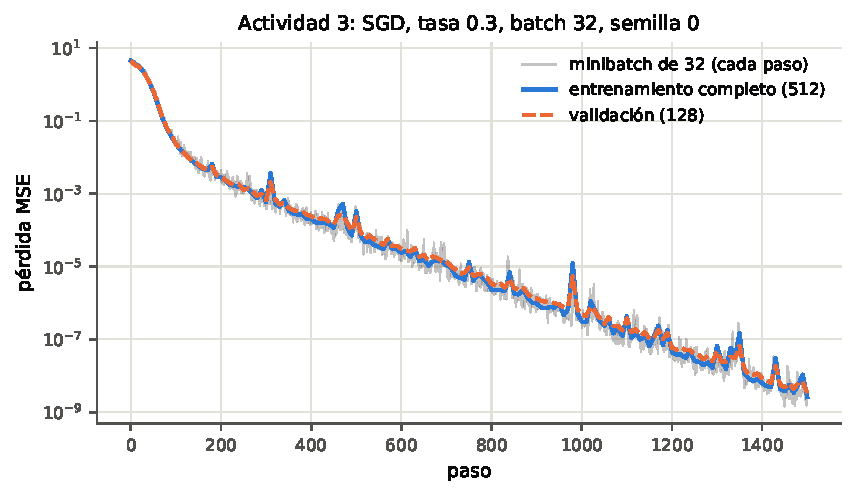
\includegraphics[width=0.72\linewidth]{act3_curvas_entrenamiento.pdf}
  \caption{Pérdida del minibatch en cada paso y pérdida en todo el conjunto de entrenamiento y de
  validación cada 10 pasos. Datos: \texttt{resultados/actividad3/registro\_entrenamiento.csv}.}
  \label{fig:act3curvas}
\end{figure}

\begin{table}[H]
  \centering\small
  \caption{Pérdida MSE antes y después de entrenar (\texttt{resultados/actividad3/resumen.json}).
  Aquí no se eligen hiperparámetros, así que se informa también la prueba.}
  \label{tab:perdidas3}
  \begin{tabular}{lccc}
    \toprule
    & entrenamiento & validación & prueba \\
    \midrule
    inicial & \V{a3.perdidas.inicial.entrenamiento} & \V{a3.perdidas.inicial.validacion} & \V{a3.perdidas.inicial.prueba} \\
    final   & \V{a3.perdidas.final.entrenamiento} & \V{a3.perdidas.final.validacion} & \V{a3.perdidas.final.prueba} \\
    \bottomrule
  \end{tabular}
\end{table}

La pérdida baja unos nueve órdenes de magnitud (figura~\ref{fig:act3curvas}). La validación sigue a
la de entrenamiento durante todo el entrenamiento y la prueba queda en el mismo orden: no hay
sobreajuste, lo esperable con un profesor sin ruido, 192 parámetros y $512\cdot4\cdot8 = 16\,384$
valores objetivo. Hay saltos aislados de la pérdida (de uno a dos órdenes) de los que el
entrenamiento se recupera en pocos pasos; la Actividad 4 los relaciona con la curvatura.

\textbf{Los pesos cambian.} La tabla~\ref{tab:cambio} y la figura~\ref{fig:act3cambio} (Anexo~\ref{anx:figuras}) muestran que
las tres matrices se alejan de su valor inicial durante los primeros 400 pasos ($W_V$ antes que
$W_Q$ y $W_K$) y luego se estabilizan;
el Anexo~\ref{anx:figuras} muestra las matrices antes y después.

\begin{table}[H]
  \centering\small
  \caption{Cambio de los pesos (\texttt{resultados/actividad3/resumen.json}, \texttt{pesos.json}).}
  \label{tab:cambio}
  \begin{tabular}{lcccc}
    \toprule
    & $\|W_0\|_F$ & $\|W_{\text{final}}\|_F$ & $\|W_{\text{final}}-W_0\|_F$ & cambio relativo \\
    \midrule
    $W_Q$ & \V{a3.cambio_pesos.W_Q.norma_F_inicial} & \V{a3.cambio_pesos.W_Q.norma_F_final} & \V{a3.cambio_pesos.W_Q.norma_F_cambio} & \V{a3.cambio_pesos.W_Q.cambio_relativo} \\
    $W_K$ & \V{a3.cambio_pesos.W_K.norma_F_inicial} & \V{a3.cambio_pesos.W_K.norma_F_final} & \V{a3.cambio_pesos.W_K.norma_F_cambio} & \V{a3.cambio_pesos.W_K.cambio_relativo} \\
    $W_V$ & \V{a3.cambio_pesos.W_V.norma_F_inicial} & \V{a3.cambio_pesos.W_V.norma_F_final} & \V{a3.cambio_pesos.W_V.norma_F_cambio} & \V{a3.cambio_pesos.W_V.cambio_relativo} \\
    \bottomrule
  \end{tabular}
\end{table}


\textbf{Comparación con el profesor.} No es necesario recuperar las matrices originales, y de hecho
$W_Q$ no se recupera: su error relativo frente a $W_Q^*$ es
\V{a3.comparacion_profesor.error_relativo_W_Q}. En cambio $W_QW_K^\top$ coincide con
$W_Q^*W_K^{*\top}$ con error relativo \V{a3.comparacion_profesor.error_relativo_W_Q_W_KT}, y $W_V$
con $W_V^*$ con error \V{a3.comparacion_profesor.error_relativo_W_V} (figura~\ref{fig:profesor}).
Es lo que predice la sección 2.4: $S$ solo depende de $M = W_QW_K^\top$, y para toda $R\in\R^{8\times8}$
invertible $(W_QR)(W_KR^{-\top})^\top = M$, así que hay una familia de dimensión
$\dim GL(8) = 64$ de parametrizaciones equivalentes. El hessiano de la pérdida en los pesos del
profesor lo confirma: tiene exactamente \V{curv.n_valores_propios_casi_nulos_profesor} valores
propios casi nulos ($|\lambda|\le\V{curv.mayor_abs_casi_nulo_profesor}$), separados por cinco órdenes
de magnitud del menor valor propio positivo, \V{curv.menor_valor_propio_no_nulo_profesor}
(\texttt{resultados/actividad4/curvatura.json}). $W_V$, en cambio, entra linealmente en $H$ y queda
determinada por los datos.

\begin{figure}[tbp]
  \centering
  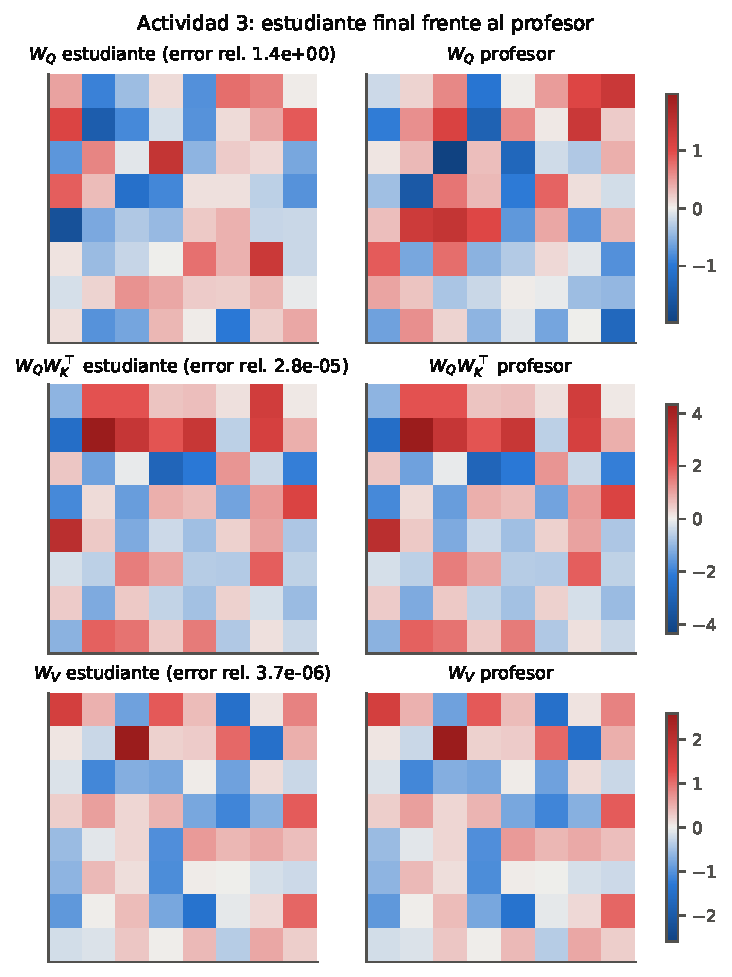
\includegraphics[width=0.42\linewidth]{act3_comparacion_profesor.pdf}
  \caption{Estudiante final frente al profesor (\texttt{pesos.json}). $W_Q$ difiere, pero
  $W_QW_K^\top$ y $W_V$ coinciden.}
  \label{fig:profesor}
\end{figure}

\subsection{Prueba de gradientes}
\path{codigo/actividad3_gradientes.py} compara, en float64, el gradiente de autograd con la
diferencia central $(L(w+\varepsilon)-L(w-\varepsilon))/(2\varepsilon)$ para tres entradas al azar de
cada matriz (semilla 11) y luego para las 192. Todas las evaluaciones usan el mismo minibatch de 32
ejemplos (semilla 7) y los pesos iniciales de la semilla 0; solo cambia la entrada $w$. Se divide por
la diferencia efectivamente representable $(w+\varepsilon)-(w-\varepsilon)$, no por $2\varepsilon$.

\textbf{Elección de $\varepsilon$.} El error de truncamiento de la diferencia central es
$\varepsilon^2|L'''|/6$ y el de redondeo es del orden de $u|L|/\varepsilon$, con $u$ el épsilon de
máquina. La suma es mínima en $\varepsilon^*\approx(3u|L|/|L'''|)^{1/3}$, del orden de $u^{1/3}$ si
$L$ y $L'''$ son de orden 1 (los pesos tienen entradas de tamaño $\approx0{,}35$, así que no hace
falta escalar). Se usa $\varepsilon = u^{1/3} = \V{g.por_tipo.float64.eps_elegido}$ en float64; el
error absoluto esperado es del orden de $u^{2/3}|L|\approx 3{,}7\cdot10^{-11}\cdot
\V{g.por_tipo.float64.perdida_minibatch}\approx 1{,}7\cdot10^{-10}$.

\textbf{Resultados} (\texttt{resultados/gradientes/}). En las 9 entradas, el error relativo máximo es
\V{g.por_tipo.float64.error_rel_max_9_entradas} y el absoluto máximo
\V{g.por_tipo.float64.error_abs_max_9_entradas}. En las 192 entradas, el error absoluto máximo es
\V{g.por_tipo.float64.todas_las_192_entradas.error_abs_max}, del orden previsto, y el error relativo
del vector completo es \V{g.por_tipo.float64.todas_las_192_entradas.error_rel_norma}
($\|\nabla L\| = \V{g.por_tipo.float64.todas_las_192_entradas.norma_gradiente}$). Los errores
relativos más altos aparecen en entradas con gradiente pequeño (el menor $|\partial L/\partial w|$ es
\V{g.por_tipo.float64.todas_las_192_entradas.abs_grad_min}), donde un error absoluto de
$10^{-10}$ pesa más. El barrido de la figura~\ref{fig:grad} tiene la forma en V esperada: para
$\varepsilon$ grande el error cae como $\varepsilon^2$ (cuatro órdenes entre $10^{-1}$ y $10^{-3}$),
para $\varepsilon$ pequeño crece como $1/\varepsilon$, y el mínimo de la mediana está en
$\varepsilon = \V{g.por_tipo.float64.eps_con_menor_mediana}$, junto al valor elegido. Las entradas de
$W_V$ no tienen error de truncamiento, porque $L$ es cuadrática en $W_V$ ($L'''=0$), y su error sigue
bajando con $\varepsilon$. En float32 ($u\approx1{,}2\cdot10^{-7}$) el mejor error relativo es del
orden de $10^{-3}$--$10^{-4}$ y por debajo de $\varepsilon\approx10^{-7}$ la diferencia de pérdidas se
redondea a cero: float32 no basta para validar gradientes con precisión.

\begin{figure}[tbp]
  \centering
  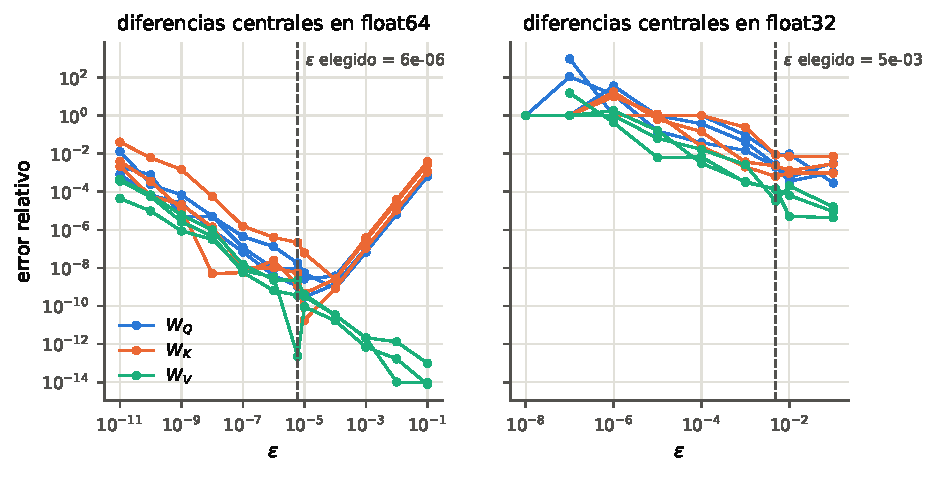
\includegraphics[width=0.74\linewidth]{gradientes_error_vs_epsilon.pdf}
  \caption{Error relativo $|g_{\text{autograd}}-g_{\text{dif}}|/|g_{\text{autograd}}|$ de 9 entradas
  según $\varepsilon$ (\texttt{gradientes\_barrido\_eps.csv}). Línea discontinua: $\varepsilon=u^{1/3}$.}
  \label{fig:grad}
\end{figure}

% ============================================================================================
\section{Actividad 4: comparación de optimizadores}

\subsection{Diseño controlado}
Todas las corridas (\path{codigo/actividad4_experimentos.py}) usan la cabeza, los datos y la división
de la Actividad 3. Para cada semilla $s\in\{0,1,2\}$, la inicialización del estudiante y el orden de
los minibatches son idénticos en todas las configuraciones, y el presupuesto es el mismo: 1500 pasos
con batch 32. Se entrenan 10 configuraciones con 3 semillas cada una (30 corridas, unos 2,5 minutos
en 2 CPU, incluidos 34 hessianos):
\begin{itemize}[nosep]
  \item \textbf{SGD} (sin momento) con $\eta\in\{0{,}03;\,0{,}1;\,0{,}3;\,1;\,3\}$: rejilla logarítmica
        alrededor de $2/\lambda_{\max}$, que vale $\approx\V{curv.limite_estabilidad_gd_inicial.mediana}$
        en la inicialización ($\lambda_{\max}=\V{curv.lambda_max_inicial.mediana}$) y
        $\approx\V{curv.limite_estabilidad_gd_profesor}$ en el profesor
        ($\lambda_{\max}=\V{curv.lambda_max_profesor}$).
  \item \textbf{Adam} ($\beta=(0{,}9;\,0{,}999)$) con $\eta\in\{0{,}001;\,0{,}003;\,0{,}01;\,0{,}03;\,0{,}1\}$.
        Adam mueve cada entrada aproximadamente $\eta$ por paso, sin importar la escala del gradiente
        (el primer paso mide exactamente $\eta\sqrt{192}$: cociente medido
        \V{deriv.adam_primer_paso_cociente_min}). Con pesos de tamaño $\approx0{,}35$, la rejilla va
        desde el valor por defecto $10^{-3}$ (0,3\,\% por paso) hasta $0{,}1$ (30\,\%).
\end{itemize}
\textbf{Selección y prueba.} Para cada optimizador se elige la tasa con menor media entre semillas
de $\log_{10}$ de la pérdida de validación final (el logaritmo evita que una semilla domine una media
de valores que difieren en órdenes de magnitud). Solo después se evalúan en prueba las tasas elegidas,
leyendo los pesos guardados (\texttt{seleccion.json}, \texttt{pesos\_finales.json},
\texttt{prueba.csv}). La tabla~\ref{tab:act4} resume las 30 corridas.

\begin{table}[H]
  \centering
  \caption{Configuraciones y métricas (mediana [mínimo, máximo] entre 3 semillas; columnas sin rango:
  mediana). $\|\nabla L\|$ final: media de los últimos 50 pasos. $\lambda_{\max}$: hessiano de la
  pérdida de entrenamiento al final. En negrita, la tasa elegida por validación. Datos:
  \texttt{resultados/actividad4/corridas.csv} y \texttt{prueba.csv}.}
  \label{tab:act4}
  \resizebox{\linewidth}{!}{\begin{tabular}{llccccccc}
\toprule
Opt. & $\eta$ & $L_{\mathrm{val}}$ final & $L_{\mathrm{ent}}$ final & $L_{\mathrm{val}}$ final/mín & pasos a $L_{\mathrm{val}}<10^{-2}$ & $\|\nabla L\|$ final & $\lambda_{\max}$ final & $L_{\mathrm{prueba}}$ (elegidas) \\
\midrule
SGD & \num{0.03} & \num{4.53e-03} [\num{3.82e-03}, \num{6.52e-03}] & \num{3.75e-03} & \num{1} & \num{1130} & \num{5.76e-02} & \num{3.15} &  \\
SGD & \num{0.1} & \num{1.32e-04} [\num{2.77e-05}, \num{9.67e-04}] & \num{9.76e-05} & \num{1} & \num{340} & \num{1.53e-02} & \num{3.19} &  \\
SGD & \textbf{\num{0.3}} & \num{2.95e-08} [\num{3.39e-09}, \num{5.68e-04}] & \num{2.13e-08} & \num{1} & \num{120} & \num{5.54e-04} & \num{3.15} & \num{2.58e-08} [\num{4.21e-09}, \num{3.00e-04}] \\
SGD & \num{1} & \num{4.59e-02} [\num{2.90e-02}, \num{7.16e-02}] & \num{4.91e-02} & \num{5.05} & 2/3 alcanzan & \num{5.67e-01} & \num{2.00} &  \\
SGD & \num{3} & \num{1.64e+00} [\num{9.79e-01}, \num{2.10e+00}] & \num{1.70e+00} & \num{2.49} & 0/3 alcanzan & \num{6.11e-01} & \num{4.36} &  \\
\midrule
Adam & \num{0.001} & \num{1.63e-01} [\num{7.51e-02}, \num{2.45e-01}] & \num{1.63e-01} & \num{1} & 0/3 alcanzan & \num{3.13e-01} & \num{2.46} &  \\
Adam & \textbf{\num{0.003}} & \num{2.71e-04} [\num{1.70e-04}, \num{3.71e-04}] & \num{3.80e-04} & \num{1} & \num{920} & \num{1.96e-02} & \num{3.06} & \num{2.98e-04} [\num{1.58e-04}, \num{3.50e-04}] \\
Adam & \num{0.01} & \num{1.05e-03} [\num{5.88e-06}, \num{4.33e-03}] & \num{1.57e-03} & \num{6.7} & \num{280} & \num{1.08e-01} & \num{2.83} &  \\
Adam & \num{0.03} & \num{7.72e-03} [\num{5.29e-03}, \num{2.21e-02}] & \num{8.15e-03} & \num{1.66} & \num{190} & \num{2.29e-01} & \num{2.37} &  \\
Adam & \num{0.1} & \num{1.43e-01} [\num{1.01e-01}, \num{1.83e-01}] & \num{1.37e-01} & \num{2.2} & 0/3 alcanzan & \num{6.34e-01} & \num{2.09} &  \\
\bottomrule
\end{tabular}
}
\end{table}

\subsection{Experimento A: tasa de aprendizaje con SGD}
\begin{figure}[tbp]
  \centering
  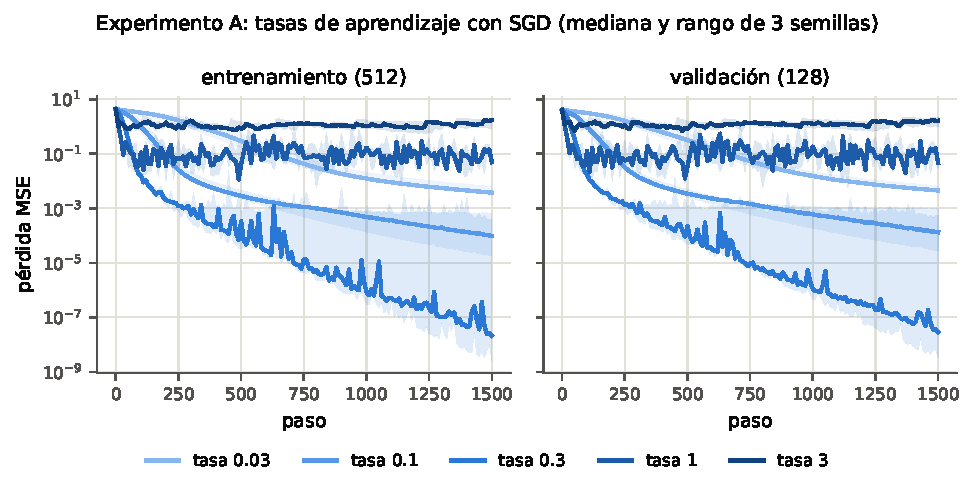
\includegraphics[width=0.82\linewidth]{act4_A_sgd_tasas.pdf}
  \caption{SGD con cinco tasas: mediana (línea) y rango (banda) de 3 semillas
  (\texttt{registro\_pasos.csv}).}
  \label{fig:A}
\end{figure}
Con $\eta = 0{,}03$ y $0{,}1$ el descenso es prácticamente monótono (pérdida final igual o muy
cercana a la mínima) pero lento:
la validación baja de $10^{-2}$ en \V{tab.sgd.0.03.pasos_val_menor_umbral} y
\V{tab.sgd.0.1.pasos_val_menor_umbral} pasos (medianas). Con $\eta=0{,}3$ lo logra en
\V{tab.sgd.0.3.pasos_val_menor_umbral} pasos y termina en \V{tab.sgd.0.3.val_final}: es la tasa
elegida. Su rango es amplio: con la semilla 2, SGD se estanca cerca de $10^{-3}$ tanto con
$\eta=0{,}3$ (\V{run.sgd.0.3.2.perdida_validacion_final}) como con $\eta=0{,}1$
(\V{run.sgd.0.1.2.perdida_validacion_final}), y con $\eta=0{,}3$ su norma del gradiente se queda en
\V{run.sgd.0.3.2.norma_grad_media_ultimos_50}, frente a \V{run.sgd.0.3.0.norma_grad_media_ultimos_50}
con la semilla 0. La mediana sola ocultaría esa sensibilidad a la inicialización.

Con $\eta=1$ la pérdida cae rápido al principio, pero luego oscila entre $10^{-2}$ y $10^{-1}$ sin
converger: la pérdida final es \V{tab.sgd.1.val_final_sobre_min} veces la mínima alcanzada y la norma
del gradiente se mantiene en \V{tab.sgd.1.norma_grad_final}. Con $\eta=3$ se estanca: termina con
pérdida de entrenamiento \V{tab.sgd.3.ent_final} (mediana), del orden de predecir cero, y la mejor
validación de las tres semillas es \V{run.sgd.3.0.perdida_validacion_min}; aun así no diverge
numéricamente (no hay \texttt{nan} ni infinitos).

\textbf{Estabilidad y curvatura.} El límite de estabilidad relevante no es el de la inicialización
($2/\lambda_{\max}\approx3{,}7$, que admitiría $\eta=1$) sino el de la región a la que llega el
entrenamiento: la curvatura crece de $\lambda_{\max}\approx\V{curv.lambda_max_inicial.mediana}$ al
inicio a \V{tab.sgd.0.3.lambda_max_final} en los mínimos que alcanzan las corridas estables, y
$2/3{,}15\approx0{,}63$ queda entre $0{,}3$ y $1$, justo donde cambia el comportamiento. Las corridas
con $\eta=1$ terminan con $\lambda_{\max}$ = \V{run.sgd.1.0.lambda_max_final},
\V{run.sgd.1.1.lambda_max_final} y \V{run.sgd.1.2.lambda_max_final}, alrededor de $2/\eta = 2$
(figura~\ref{fig:curv}): el descenso por gradiente con paso $\eta$ solo es estable donde
$\lambda_{\max}\lesssim2/\eta$, y como los mínimos tienen curvatura mayor, la iteración se queda
oscilando en ese borde, un comportamiento conocido como \emph{borde de estabilidad} (Cohen et al.,
2021). Es una interpretación compatible con estas mediciones, no una demostración: se midió el
hessiano de la pérdida completa al final, no a lo largo de la trayectoria. Los saltos aislados con
$\eta=0{,}3$ son coherentes con minibatches cuya curvatura local supera brevemente ese límite.

\begin{figure}[tbp]
  \centering
  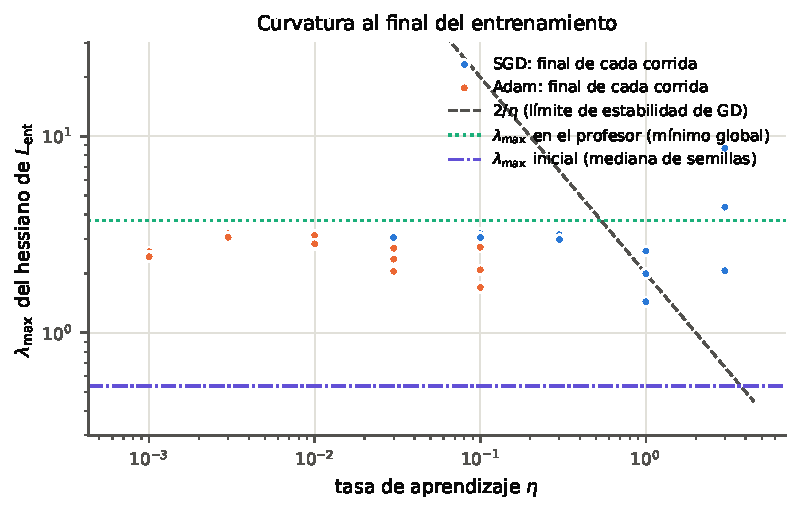
\includegraphics[width=0.58\linewidth]{act4_curvatura.pdf}
  \caption{Mayor valor propio del hessiano al final de cada corrida frente a $\eta$
  (\texttt{corridas.csv}, \texttt{curvatura.json}).}
  \label{fig:curv}
\end{figure}

\subsection{Experimento B: SGD frente a Adam}
\begin{figure}[tbp]
  \centering
  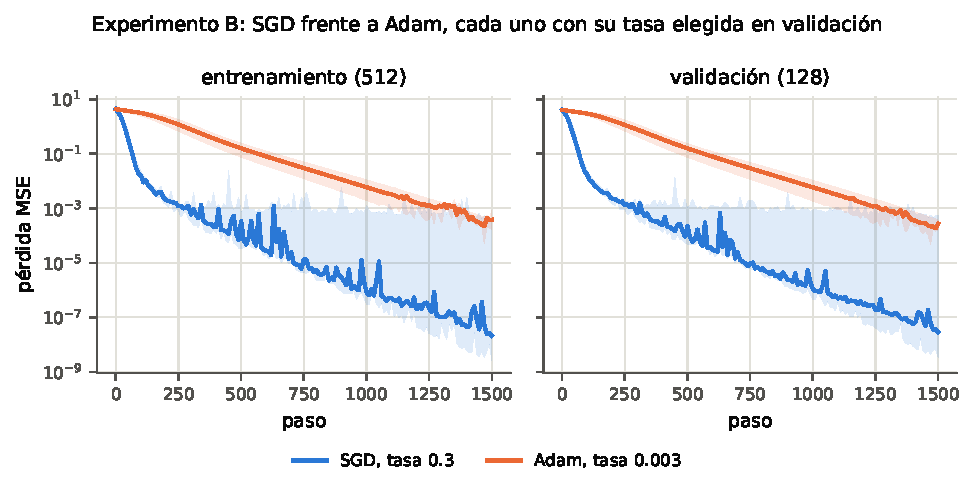
\includegraphics[width=0.82\linewidth]{act4_B_sgd_vs_adam.pdf}
  \caption{SGD ($\eta=\V{sel.seleccion.sgd.tasa}$) frente a Adam ($\eta=\V{sel.seleccion.adam.tasa}$),
  cada uno con su tasa elegida en validación; mediana y rango de 3 semillas. Las curvas de las cinco
  tasas de Adam están en el Anexo~\ref{anx:figuras}.}
  \label{fig:B}
\end{figure}
\textbf{Tasas.} Cada optimizador usa la tasa elegida en su propia rejilla, porque sus escalas no son
comparables: el paso de SGD es $\eta\|\nabla L\|$ y el de Adam es del orden de $\eta$ por entrada. En
Adam la elección es casi un empate: la media de $\log_{10}$ de la validación final es
\V{sel.puntajes.adam.0.003} con $\eta = 0{,}003$ y \V{sel.puntajes.adam.0.01} con $\eta=0{,}01$.
$\eta=0{,}01$ llega antes a $10^{-2}$ (\V{tab.adam.0.01.pasos_val_menor_umbral} frente a
\V{tab.adam.0.003.pasos_val_menor_umbral} pasos) y con la semilla 0 alcanza
\V{run.adam.0.01.0.perdida_validacion_min}, pero en las tres semillas termina por encima de su mínimo
(cociente mediano \V{tab.adam.0.01.val_final_sobre_min}): con tasa constante, Adam sigue dando pasos
de tamaño $\approx\eta$ cerca del mínimo y oscila. Con $\eta = 0{,}003$ termina en su mínimo en 2 de
3 semillas; con la semilla 1 sube al final de \V{run.adam.0.003.1.perdida_validacion_min} a
\V{run.adam.0.003.1.perdida_validacion_final}. Con $\eta=0{,}001$ es demasiado lento para el
presupuesto y con $\eta \ge 0{,}03$ se estanca.

\textbf{Comparación.} Con el mismo presupuesto, SGD ($\eta=0{,}3$) termina con pérdida de validación
\V{tab.sgd.0.3.val_final} y Adam ($\eta=0{,}003$) con \V{tab.adam.0.003.val_final}. En prueba, SGD
obtiene \V{tab.sgd.0.3.prueba} y Adam \V{tab.adam.0.003.prueba}. Por semilla, SGD queda varios
órdenes por debajo con las semillas 0 y 1 (\V{prueba.sgd.0} y \V{prueba.sgd.1} frente a
\V{prueba.adam.0} y \V{prueba.adam.1}); con la semilla 2, en la que SGD se estanca, Adam queda algo
mejor (\V{prueba.adam.2} frente a \V{prueba.sgd.2}). La ventaja de SGD aquí es razonable: el
problema es pequeño, sin ruido y realizable, de modo que en la solución se anulan los gradientes de
todos los ejemplos y el paso de SGD, proporcional al gradiente, se achica solo; Adam normaliza el
gradiente y necesita una tasa pequeña para no oscilar, lo que lo hace más lento al principio. No se
puede generalizar a otros problemas: Adam suele rendir mejor con gradientes ruidosos o de escalas muy
distintas entre parámetros, y aquí no se probó Adam con decaimiento de la tasa, que probablemente
reduciría su oscilación final.

\subsection{Experimento C: norma del gradiente}
\begin{figure}[tbp]
  \centering
  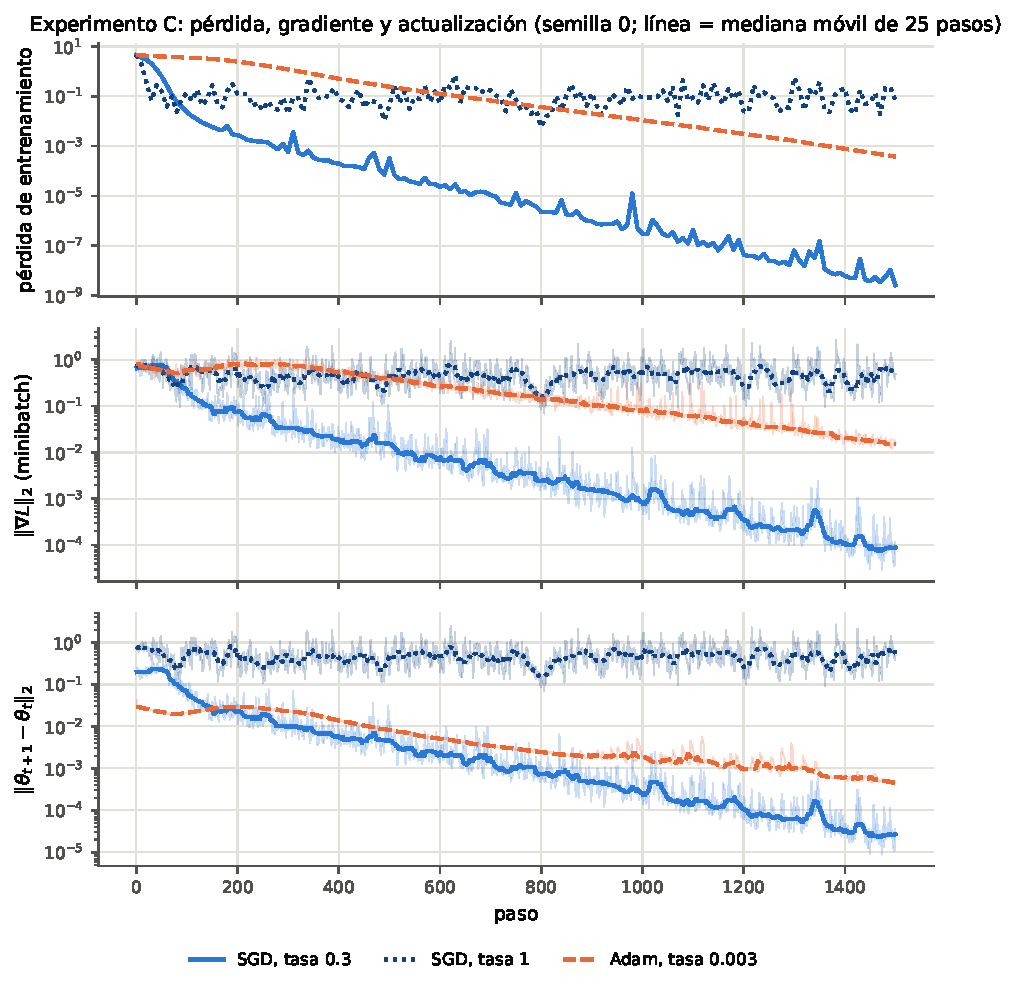
\includegraphics[width=0.6\linewidth]{act4_C_dinamica.pdf}
  \caption{Pérdida de entrenamiento, norma del gradiente y norma de la actualización para la semilla 0
  (\texttt{registro\_pasos.csv}).}
  \label{fig:Cdin}
\end{figure}
La norma del gradiente se registra en cada paso de las 30 corridas, junto con la de la actualización
$\|\theta_{t+1}-\theta_t\|$. En SGD ambas son proporcionales: el registro da
$\|\theta_{t+1}-\theta_t\| = \eta\|\nabla L\|$ con desvío relativo máximo de
\V{deriv.sgd_desvio_rel_max_actualizacion}, atribuible al redondeo de float32. Con $\eta=0{,}3$ la
norma baja de \V{run.sgd.0.3.0.norma_grad_inicial} a \V{run.sgd.0.3.0.norma_grad_media_ultimos_50}
(semilla 0) y los pasos se achican con ella, mientras la pérdida baja en paralelo en escala
logarítmica (figura~\ref{fig:Cdin}); los saltos de la pérdida van acompañados de picos de la norma
(por ejemplo, cerca del paso 1350). Con $\eta = 1$ y $3$ la norma se mantiene entre $0{,}3$ y $0{,}7$
durante toda la corrida (figura~\ref{fig:Cnorma}, Anexo~\ref{anx:figuras}): los pasos siguen siendo grandes y la pérdida no
converge. En Adam el paso no es proporcional al gradiente: el primero mide $\eta\sqrt{192}$ sin importar
$\|\nabla L\|$, y los siguientes dependen del cociente entre los promedios móviles del gradiente y de su
cuadrado. Con $\eta=0{,}003$ la norma del gradiente cae de forma sostenida hasta
\V{tab.adam.0.003.norma_grad_final}; con $\eta\ge0{,}01$ se estanca en un nivel que crece con $\eta$,
reflejo de la oscilación alrededor del mínimo. Una norma del gradiente que no decrece es, en estos experimentos, la señal más
temprana de una tasa demasiado grande.

\subsection{Conclusiones y limitaciones}
\begin{itemize}[nosep]
  \item La tasa controla el compromiso entre velocidad y estabilidad: para SGD, la mejor tasa ($0{,}3$)
        está cerca del límite $2/\lambda_{\max}$ de los mínimos, no del de la inicialización.
  \item Con su tasa elegida en validación, SGD fue más rápido y varios órdenes más preciso que Adam
        en 2 de 3 semillas; en la tercera, donde SGD se estancó, Adam fue algo mejor.
  \item No hubo sobreajuste en ninguna configuración (validación y entrenamiento coinciden); los
        problemas observados son de convergencia: estancamiento con la semilla 2 y oscilación con
        tasas grandes.
  \item Limitaciones: un solo problema sintético, 3 semillas (los rangos son mínimo y máximo, no
        intervalos de confianza), presupuesto fijo, sin momento ni decaimiento de la tasa, y una
        selección de Adam muy cercana al empate. La selección usa la validación final; con
        detención temprana el resultado de Adam podría cambiar.
\end{itemize}

% ============================================================================================
\section{Actividad 5: auditoría y validación humana}
\pendiente{Iniciar una sesión \emph{nueva} del agente auditor (sin la conversación de desarrollo),
que ejecute en el contenedor \texttt{auditoria} y escriba solo en \texttt{auditoria/}. Pedirle que
revise derivaciones, código, pruebas de gradientes, métricas y conclusiones, que reejecute los
comandos de \texttt{parte1/README.md} con \texttt{--salida /workspace/auditoria/verificaciones/...}
y que genere \texttt{auditoria/HANDOFF\_P1.md}. Conservar su informe y registrar su prompt en
\texttt{auditoria/PROMPTS.md}. Luego verificar personalmente sus observaciones y registrar en
\texttt{auditoria/VALIDACION\_HUMANA.md} qué se aceptó o rechazó y por qué. Resumir aquí los hallazgos
y las decisiones.}

% ============================================================================================
\section{Uso de agentes y trazabilidad}
Los prompts de la Parte 0 están en \path{parte1/PROMPTS.md} (entradas P1-01 a P1-08) y los de esta
sesión de teoría en la serie P1-T de ese mismo archivo. La sesión de teoría escribió el código, ejecutó
los experimentos en el contenedor \texttt{teoria}, generó las figuras desde los registros y redactó
este borrador; no eligió matrices ni calculó los ejercicios manuales. Cada número de las Actividades 3
y 4 se inserta desde los registros con \path{codigo/valores_informe.py}, y cada figura se regenera con
\path{codigo/regenerar_figuras.py}; una reejecución completa en el mismo contenedor reprodujo bit a bit
los registros, pesos, tablas y figuras.
\pendiente{Revisión personal de este borrador por los integrantes: derivaciones, interpretación de
resultados y redacción.}

% ============================================================================================
\section*{Referencias}
\addcontentsline{toc}{section}{Referencias}
\begin{enumerate}[nosep, label={[\arabic*]}]
  \item Vaswani, A. et al. (2017). Attention Is All You Need. \url{https://arxiv.org/abs/1706.03762}
  \item Kingma, D. P. y Ba, J. (2014). Adam: A Method for Stochastic Optimization.
        \url{https://arxiv.org/abs/1412.6980}
  \item Loshchilov, I. y Hutter, F. (2019). Decoupled Weight Decay Regularization.
        \url{https://arxiv.org/abs/1711.05101}
  \item Cohen, J. M., Kaur, S., Li, Y., Kolter, J. Z. y Talwalkar, A. (2021). Gradient Descent on
        Neural Networks Typically Occurs at the Edge of Stability. ICLR 2021.
  \item Nocedal, J. y Wright, S. J. (2006). \emph{Numerical Optimization}, 2.ª ed. Springer
        (diferencias finitas y elección del paso).
  \item PyTorch. Automatic Differentiation. \url{https://docs.pytorch.org/docs/stable/autograd.html}
  \item Docker. Compose File Reference y Bind Mounts. \url{https://docs.docker.com/reference/compose-file/services/}
\end{enumerate}

\appendix
\section{Desarrollo manual escaneado}\label{anx:escaneo}
\pendiente{Escaneo o fotografía legible del desarrollo manual de las Actividades 1 y 2, identificado
por su autor.}

\section{Figuras complementarias}\label{anx:figuras}
\begin{figure}[H]
  \centering
  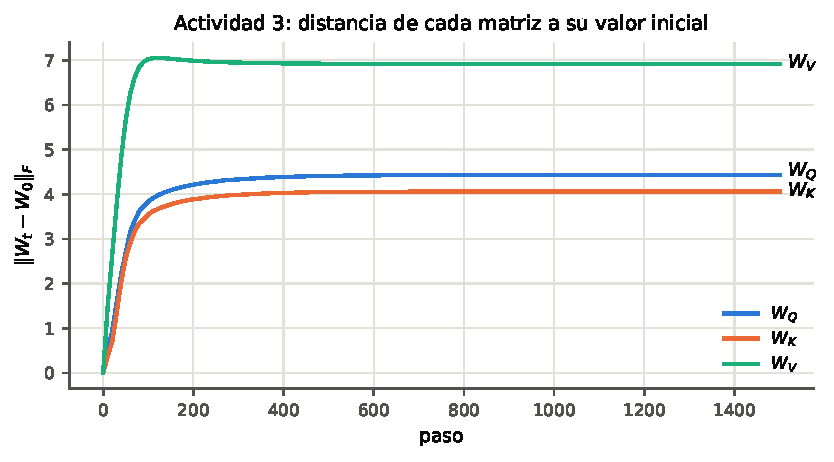
\includegraphics[width=0.78\linewidth]{act3_cambio_pesos.pdf}
  \caption{Distancia de cada matriz a su valor inicial, cada 10 pasos (\texttt{registro\_entrenamiento.csv}).}
  \label{fig:act3cambio}
\end{figure}
\begin{figure}[H]
  \centering
  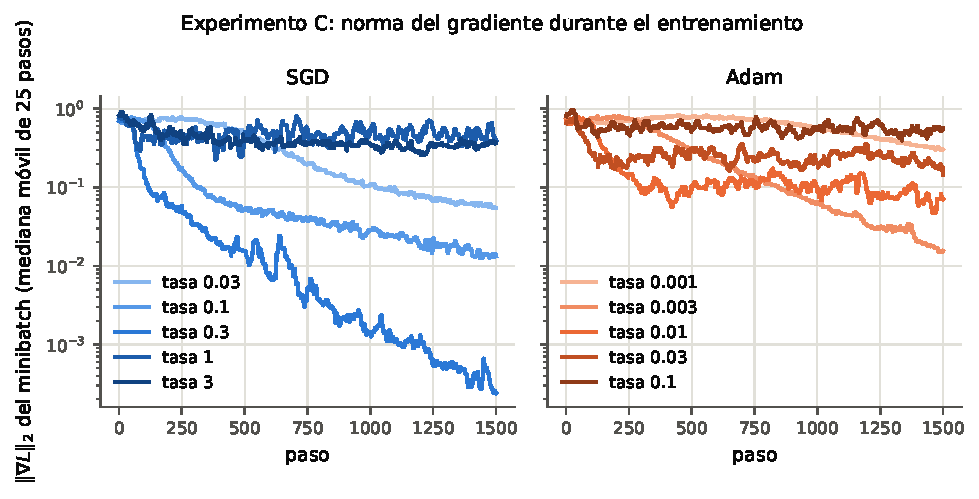
\includegraphics[width=0.9\linewidth]{act4_C_norma_gradiente.pdf}
  \caption{Norma del gradiente del minibatch, mediana móvil de 25 pasos y mediana de 3 semillas
  (\texttt{registro\_pasos.csv}).}
  \label{fig:Cnorma}
\end{figure}
\begin{figure}[tbp]
  \centering
  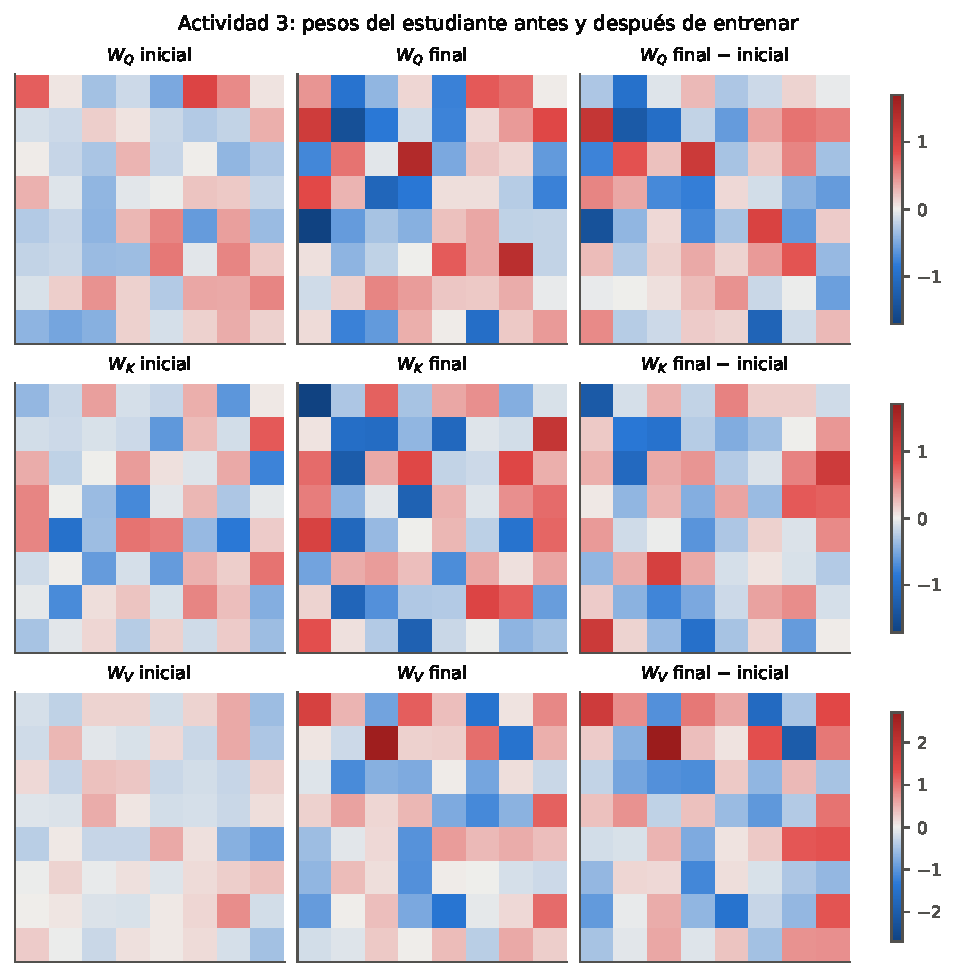
\includegraphics[width=0.62\linewidth]{act3_pesos_antes_despues.pdf}
  \caption{Actividad 3: matrices del estudiante al inicio, al final y su diferencia (\texttt{pesos.json}).}
\end{figure}
\begin{figure}[tbp]
  \centering
  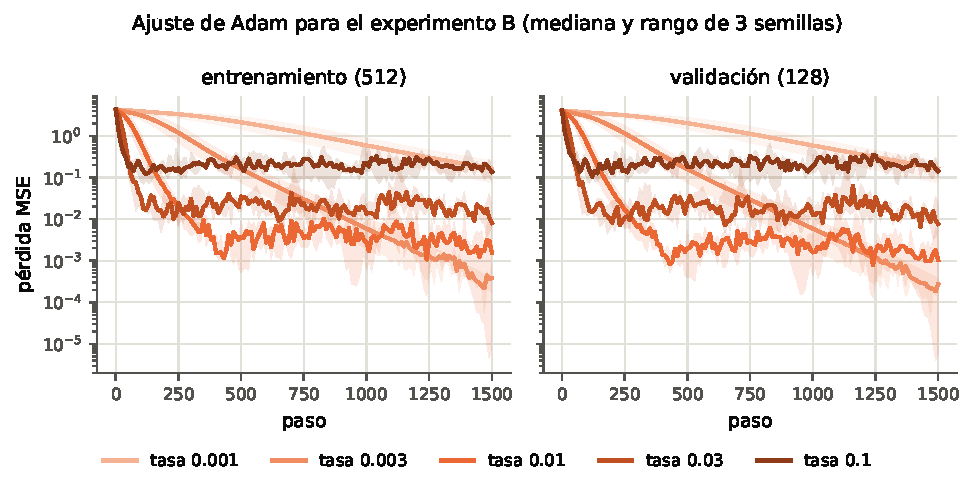
\includegraphics[width=0.9\linewidth]{act4_B_adam_tasas.pdf}
  \caption{Adam con cinco tasas, base de la elección para el experimento B (\texttt{registro\_pasos.csv}).}
\end{figure}

\section{Comandos de reproducción}\label{anx:comandos}
Desde \path{tp2-transformers/} (detalles y comandos del auditor en \path{parte1/README.md}):
\begin{verbatim}
docker compose exec teoria python -m unittest discover -s codigo -p "test_*.py" -v
docker compose exec teoria python codigo/actividad3_entrenar.py
docker compose exec teoria python codigo/actividad3_gradientes.py
docker compose exec teoria python codigo/actividad4_experimentos.py
docker compose exec teoria python codigo/regenerar_figuras.py
docker compose exec teoria python codigo/valores_informe.py
cd parte1/informe && latexmk -pdf informe.tex
\end{verbatim}

\end{document}
